% Options for packages loaded elsewhere
\PassOptionsToPackage{unicode}{hyperref}
\PassOptionsToPackage{hyphens}{url}
%
\documentclass[
]{article}
\usepackage{amsmath,amssymb}
\usepackage{lmodern}
\usepackage{iftex}
\ifPDFTeX
  \usepackage[T1]{fontenc}
  \usepackage[utf8]{inputenc}
  \usepackage{textcomp} % provide euro and other symbols
\else % if luatex or xetex
  \usepackage{unicode-math}
  \defaultfontfeatures{Scale=MatchLowercase}
  \defaultfontfeatures[\rmfamily]{Ligatures=TeX,Scale=1}
\fi
% Use upquote if available, for straight quotes in verbatim environments
\IfFileExists{upquote.sty}{\usepackage{upquote}}{}
\IfFileExists{microtype.sty}{% use microtype if available
  \usepackage[]{microtype}
  \UseMicrotypeSet[protrusion]{basicmath} % disable protrusion for tt fonts
}{}
\makeatletter
\@ifundefined{KOMAClassName}{% if non-KOMA class
  \IfFileExists{parskip.sty}{%
    \usepackage{parskip}
  }{% else
    \setlength{\parindent}{0pt}
    \setlength{\parskip}{6pt plus 2pt minus 1pt}}
}{% if KOMA class
  \KOMAoptions{parskip=half}}
\makeatother
\usepackage{xcolor}
\usepackage[margin=1in]{geometry}
\usepackage{longtable,booktabs,array}
\usepackage{calc} % for calculating minipage widths
% Correct order of tables after \paragraph or \subparagraph
\usepackage{etoolbox}
\makeatletter
\patchcmd\longtable{\par}{\if@noskipsec\mbox{}\fi\par}{}{}
\makeatother
% Allow footnotes in longtable head/foot
\IfFileExists{footnotehyper.sty}{\usepackage{footnotehyper}}{\usepackage{footnote}}
\makesavenoteenv{longtable}
\usepackage{graphicx}
\makeatletter
\def\maxwidth{\ifdim\Gin@nat@width>\linewidth\linewidth\else\Gin@nat@width\fi}
\def\maxheight{\ifdim\Gin@nat@height>\textheight\textheight\else\Gin@nat@height\fi}
\makeatother
% Scale images if necessary, so that they will not overflow the page
% margins by default, and it is still possible to overwrite the defaults
% using explicit options in \includegraphics[width, height, ...]{}
\setkeys{Gin}{width=\maxwidth,height=\maxheight,keepaspectratio}
% Set default figure placement to htbp
\makeatletter
\def\fps@figure{htbp}
\makeatother
\setlength{\emergencystretch}{3em} % prevent overfull lines
\providecommand{\tightlist}{%
  \setlength{\itemsep}{0pt}\setlength{\parskip}{0pt}}
\setcounter{secnumdepth}{5}
\newlength{\cslhangindent}
\setlength{\cslhangindent}{1.5em}
\newlength{\csllabelwidth}
\setlength{\csllabelwidth}{3em}
\newlength{\cslentryspacingunit} % times entry-spacing
\setlength{\cslentryspacingunit}{\parskip}
\newenvironment{CSLReferences}[2] % #1 hanging-ident, #2 entry spacing
 {% don't indent paragraphs
  \setlength{\parindent}{0pt}
  % turn on hanging indent if param 1 is 1
  \ifodd #1
  \let\oldpar\par
  \def\par{\hangindent=\cslhangindent\oldpar}
  \fi
  % set entry spacing
  \setlength{\parskip}{#2\cslentryspacingunit}
 }%
 {}
\usepackage{calc}
\newcommand{\CSLBlock}[1]{#1\hfill\break}
\newcommand{\CSLLeftMargin}[1]{\parbox[t]{\csllabelwidth}{#1}}
\newcommand{\CSLRightInline}[1]{\parbox[t]{\linewidth - \csllabelwidth}{#1}\break}
\newcommand{\CSLIndent}[1]{\hspace{\cslhangindent}#1}
\usepackage{longtable}
\usepackage{array}
\usepackage{pdflscape}
\newcommand{\blandscape}{\begin{landscape}}
\newcommand{\elandscape}{\end{landscape}}
\usepackage{float} \floatplacement{figure}{H}
\newcommand{\beginsupplement}{\setcounter{table}{0}  \renewcommand{\thetable}{S\arabic{table}} \setcounter{figure}{0} \renewcommand{\thefigure}{S\arabic{figure}}}
\ifLuaTeX
  \usepackage{selnolig}  % disable illegal ligatures
\fi
\IfFileExists{bookmark.sty}{\usepackage{bookmark}}{\usepackage{hyperref}}
\IfFileExists{xurl.sty}{\usepackage{xurl}}{} % add URL line breaks if available
\urlstyle{same} % disable monospaced font for URLs
\hypersetup{
  pdftitle={A comprehensive proteomic and bioinformatics analysis of human spinal cord injury plasma identifies proteins associated with the complement cascade and liver function as potential prognostic indicators of neurological outcome},
  pdfauthor={Gabriel Mateus Bernardo Harrington, PhD; Paul Cool, MD; Charlotte Hulme, PhD; Jessica Fisher-Stokes, MRes; Mandy Peffers, PhD; Wagih El Masri, MD; Aheed Osman, MBChB; Joy Roy Chowdhury, MBBS; Naveen Kumar, MBBS; Srinivasa Budithi, MD; Karina Wright, PhD},
  pdfkeywords={Spinal cord injury, Biomarker, Proteomics, Complement cascade},
  hidelinks,
  pdfcreator={LaTeX via pandoc}}

\title{A comprehensive proteomic and bioinformatics analysis of human spinal cord injury plasma identifies proteins associated with the complement cascade and liver function as potential prognostic indicators of neurological outcome}
\author{Gabriel Mateus Bernardo Harrington, PhD\footnote{Keele University} \and Paul Cool, MD\footnote{Robert Jones and Agnes Hunt Orthopaedic Hospital NHS Foundation Trust; Keele University} \and Charlotte Hulme, PhD \and Jessica Fisher-Stokes, MRes \and Mandy Peffers, PhD \and Wagih El Masri, MD \and Aheed Osman, MBChB \and Joy Roy Chowdhury, MBBS \and Naveen Kumar, MBBS \and Srinivasa Budithi, MD \and Karina Wright, PhD\footnote{\href{mailto:karina.wright1@nhs.net}{\nolinkurl{karina.wright1@nhs.net}}}}
\date{2022-07-12}

\begin{document}
\maketitle

\hypertarget{abstract}{%
\section{Abstract}\label{abstract}}

\hypertarget{introduction}{%
\subsection{Introduction}\label{introduction}}

Spinal Cord Injury (SCI) is a major cause of disability, with complications post-injury often leading to life-long health issues with need of extensive treatment.
Neurological outcome post-SCI can be variable and difficult to predict, particularly in incomplete injured patients.
The identification of specific SCI biomarkers in blood, may be able to improve prognostics in the field.
This study has utilised proteomic and bioinformatics methodologies to investigate differentially expressed proteins in plasma samples across human SCI cohorts with the aim of identifying prognostic biomarkers and biological pathway alterations that relate to neurological outcome.

\hypertarget{methods-and-materials}{%
\subsection{Methods and Materials}\label{methods-and-materials}}

Blood samples were taken, following informed consent, from ASIA impairment scale (AIS) grade C ``Improvers'' (those who experienced an AIS grade improvement) and ``Non-Improvers'' (No AIS change), and AIS grade A and D at \textless2 weeks (``Acute'') and approx. 3 months (``Sub-acute'') post-injury.
The total protein concentration from each sample was extracted, with pooled samples being labelled and non-pooled samples treated with ProteoMiner™ beads.
Samples were then analysed using two 4-plex isobaric tag for relative and absolute quantification (iTRAQ) analyses and a label-free experiment for comparison, before quantifying with mass spectrometry.
Data are available via ProteomeXchange with identifiers PXD035025 and PXD035072 for the iTRAQ and label-free experiments respectively.

Proteomic datasets were analysed using OpenMS (version 2.6.0).
R (version 4.1.4) and in particular, the R packages MSstats (version 4.0.1) and pathview (version 1.32.0) were used for downstream analysis.
Proteins of interest identified from this analysis were further validated by enzyme-linked immunosorbent assay (ELISA).

\hypertarget{results}{%
\subsection{Results}\label{results}}

The data demonstrated proteomic differences between the cohorts, with the results from the iTRAQ approach supporting those of the label-free analysis.
A total of 79 and 87 differentially abundant proteins across AIS and longitudinal groups were identified from the iTRAQ and label-free analyses, respectively.
Alpha-2-macroglobulin (A2M), retinol binding protein 4 (RBP4), serum amyloid A1 (SAA1), Peroxiredoxin 2, alipoprotein A1 (ApoA1) and several immunoglobulins were identified as biologically relevant and differentially abundant, with potential as individual prognostic biomarkers of neurological outcome.
Bioinformatics analyses revealed that the majority of differentially abundant proteins were components of the complement cascade and most interacted directly with the liver.

\hypertarget{conclusions}{%
\subsection{Conclusions}\label{conclusions}}

Many of the proteins of interest identified using proteomics were detected only in a single group and therefore have potential as a binary (present or absent) biomarkers, RBP4 and PRX-2 in particular.
Additional investigations into the chronology of these proteins, and their levels in other tissues (cerebrospinal fluid in particular) are needed to better understand the underlying pathophysiology, including any potentially modifiable targets.
Pathway analysis highlighted the complement cascasde as being significant across groups of differential functional recovery.

\hypertarget{introduction-1}{%
\section{Introduction}\label{introduction-1}}

Spinal cord injury (SCI) is the transient or permanent loss of normal spinal sensory, motor or autonomic function, and is a major cause of disability.
Globally, SCI affects around 500,000 people each year and is most commonly the result of road traffic accidents or falls.(Crozier-Shaw, Denton, and Morris 2020) Patients typically require extensive medical, rehabilitative and social care at high financial cost to healthcare providers. The lifetime cost of care in the UK is estimated to be £1.12 million (mean value) per SCI, with the total cost of SCI in the UK to the NHS being £1.43 billion in 2016.(McDaid et al. 2019) Individuals with SCI show markedly higher rates of mental illness relative to the general population.(Furlan, Gulasingam, and Craven 2017) Complications arising post-SCI can be long-lasting and often include pain, spasticity and cardiovascular disease, where the systemic inflammatory response that follows SCI can frequently result in organ complications, particularly in the liver and kidneys.(Gris, Hamilton, and Weaver 2008; Sun et al. 2016; Hagen 2015)

The recovery of neurological function post-SCI is highly variable, requiring any clinical trials to have an impractically large sample size to prove efficacy, hence the translation of novel efficacious therapies is challenging and expensive.(Spiess et al. 2009) Being able to more accurately predict patient outcomes would aid clinical decisions and facilitate future clinical trials.
Therefore, novel biomarkers that allow for stratification of injury severity and capacity for neurological recovery would be of high value to the field.

Biomarkers studies in SCI often investigate protein changes in cerebral spinal fluid (CSF) as the closer proximity of this medium is thought to be more reflective of the parenchymal injury.(Brian K. Kwon et al. 2019; Hulme et al. 2017) Whilst this makes CSF potentially more informative for elucidating the pathology of SCI, the repeated use of CSF for routine analysis presents challenges in clinical care due to the risk and expense associated with the invasiveness of the collection procedure.
In contrast, systemic biomarkers measurable in the blood represent a source of information that can be accessed and interpreted both a lower cost and risk.
Studies of traumatic brain injury have demonstrated that protein markers identified in CSF are also detectable in both plasma and serum.(Wang et al. 2018) More recently, circulating white blood cell populations have also been identified as potential SCI injury biomarkers, with a 2021 study showing that elevated levels of neutrophils were associated with no AIS grade conversion, while conversely an increase in lymphocytes during the first week post-SCI were associated with an AIS grade improvement.(Jogia et al. 2021)

A number of individual proteins have been shown to be altered in the bloods post-SCI, including multiple interleukins (IL), tumour necrosis factor alpha (TNF-\(\alpha\)) and C-reactive protein (CRP).(Segal et al. 1997; Hayes et al. 2002; Frost et al. 2005)

Further, changes in inflammatory marker levels detected in acute SCI patients were found to be mirrored in donor-matched blood and CSF, albeit at lower absolute concentrations systemically.(Brian K. Kwon et al. 2010)

Previously, we have shown that routinely collected blood measures associated with liver function and inflammation added predictive value to AIS motor and sensor outcomes at discharge and 12-months post-injury.(Bernardo Harrington et al. 2020; Brown et al. 2019) The current study uses an unbiased shotgun proteomic approach to investigate differentially expressed proteins in SCI patients, coupled with bioinformatics pathway and network analyses.

\hypertarget{methods-and-materials-1}{%
\section{Methods and Materials}\label{methods-and-materials-1}}

\hypertarget{patients}{%
\subsection{Patients}\label{patients}}

Blood samples were taken from SCI patients who had provided informed consent and in accordance to ethical provided by the National Research Ethics Service {[}NRES{]} Committee North West Liverpool East {[}11/NW/0876{]}.
``Improvers'' were defined as individuals who experienced an AIS grade improvement from admission to a year post-injury, whereas ``non-improvers'' were defined as patients who saw no change in AIS grade in the same period (Table \ref{tab:patient-demo-chap3}).

\begin{longtable}[t]{lll}
\caption{\label{tab:patient-demo-chap3}Patient demographics. ± denotes interquartile range}\\
\toprule
 & n & Percent\\
\midrule
\endfirsthead
\caption[]{\label{tab:patient-demo-chap3}Patient demographics. ± denotes interquartile range \textit{(continued)}}\\
\toprule
 & n & Percent\\
\midrule
\endhead

\endfoot
\bottomrule
\endlastfoot
\addlinespace[0.3em]
\multicolumn{3}{l}{\textbf{Polytrauma}}\\
\hspace{1em}Yes & 16 & 41\\
\hspace{1em}No & 23 & 59\\
\addlinespace[0.3em]
\multicolumn{3}{l}{\textbf{Gender}}\\
\hspace{1em}F & 13 & 33\\
\hspace{1em}M & 26 & 67\\
\addlinespace[0.3em]
\multicolumn{3}{l}{\textbf{Diabetes}}\\
\hspace{1em}Yes & 7 & 18\\
\hspace{1em}No & 32 & 82\\
\addlinespace[0.3em]
\multicolumn{3}{l}{\textbf{Neurological level}}\\
\hspace{1em}C & 26 & 67\\
\hspace{1em}L & 4 & 10\\
\hspace{1em}T & 9 & 23\\
\addlinespace[0.3em]
\multicolumn{3}{l}{\textbf{AIS change}}\\
\hspace{1em}A & 11 & 28\\
\hspace{1em}C & 7 & 18\\
\hspace{1em}C->D & 10 & 26\\
\hspace{1em}D & 11 & 28\\
Age at injury 
(Median years±IQR) & 53±26 & -\\*
\end{longtable}

\hypertarget{plasma-collection-and-storage}{%
\subsection{Plasma collection and storage}\label{plasma-collection-and-storage}}

Plasma samples were collected within 2 weeks of injury (acute) and at approximately 3 months post-injury (subacute).
Upon collection in EDTA (ethylenediaminetetraacetic acid) coated tubes samples were centrifuged at 600g for 15 minutes, to pellet erythrocytes and the resultant plasma fraction was aspirated and divided into aliquots for long-term storage in -80°C briefly and liquid nitrogen in the longer term.

\hypertarget{itraq-sample-prep}{%
\subsection{Sample preparation and analysis using iTRAQ proteomics}\label{itraq-sample-prep}}

Thawed plasma samples (\(2\mu l\)) each were diluted with distilled water (\(98\mu l\)).
Total protein was quantified using a Pierce™ \(660 nm\) Protein Assay (Thermo Fisher Scientific, Hemel Hempstead, UK)(Stoscheck 1987).

A total of \(100 mg\) of plasma protein was taken from each sample and pooled equally to form a patient test group.
For example, the AIS C improver group was pooled from 10 separate patient samples, 10mg of protein per patient.

The pooled plasma samples were precipitated by incubation of the sample in six times the volume of chilled acetone for 1 hour at -20°C.
The samples were then centrifuged at 6,000G for 10 minutes at 4°C, and re-suspended in \(200\mu l\) of triethylammonium bicarbonate buffer.
Sequencing Grade Modified Trypsin (\(10\mu g/85\mu g\) of protein; Promega, Madison, WI, USA) was then added to the samples for overnight digestion at 37°C.
Peptides underwent reduction and alkylation (according to the manufacturer's instructions; Applied Biosystems, Bleiswijk, The Netherlands).
Tryptic digests were labelled with iTRAQ tags (again according to the manufacturer's instructions for the iTRAQ kit), before being pooled into test groups and dried in a vacuum centrifuge.
Two individual iTRAQ experiments were set up, the first to assess acute and sub-acute improvers or non-improvers and the second to assess acute improvers and non-improvers to AIS grade A and D patients.
The following tags were used for each group of patient samples 114 tag - acute improvers, 115 tag - sub-acute improvers, 116 tag - acute non-improvers and 117 tag - sub-acute non-improvers for run 1 and 114 tag - acute improvers, 115 tag - acute non-improvers, 116 tag - AIS grade A and 117 tag - AIS grade D for run 2.

\hypertarget{itraq-mass-spectrometry-analysis}{%
\subsubsection{iTRAQ mass spectrometry analysis}\label{itraq-mass-spectrometry-analysis}}

The samples were analysed at the BSRC St.~Andrews University Mass Spectrometry and Proteomics Facility.
A total of 12 SCX fractions were analysed by nano-electrospray ionisation-liquid chromatography/tandem mass spectrometry (LC-MS/MS) using a TripleTOF 5600 tandem mass spectrometer (AB Sciex, Framingham, MA, USA) as described previously.(Fuller et al. 2015)
Each fraction (\(10 \mu l\)) was then analysed by nanoflow LC-ESI-MSMS, as described previously.

The mass spectrometry proteomics data have been deposited to the ProteomeXchange Consortium via the PRIDE partner repository with the dataset identifier PXD035025 and 10.6019/PXD035025.(Perez-Riverol et al. 2021)

\hypertarget{label-free-sample-prep}{%
\subsection{Sample preparation and analysis using label-free proteomics}\label{label-free-sample-prep}}

No sample pooling was used, and so each of the 73 samples were maintained separately throughout protein equalisation, mass spectrometry, and label-free quantification steps.
Thus, protein abundance was quantified for each sample, whereupon mean protein abundance across experimental groups was calculated to assess protein changes.

To reduce the dynamic range of proteins, ProteoMiner™ beads (BioRad, Hemel Hempstead, UK) were used.(Boschetti and Righetti 2008) Total protein was quantitated with a Pierce™ \(660 nm\) Protein Assay (Thermo Fisher Scientific, Hemel Hempstead, UK), whereupon 5 mg of total protein was applied to ProteoMiner™ beads, and processed as described previously.(Stoscheck 1987; Peffers et al. 2015)

\hypertarget{label-free-mass-spectrometry-analysis}{%
\subsubsection{Label free mass spectrometry analysis}\label{label-free-mass-spectrometry-analysis}}

Tryptic peptides were subjected to LC-MC/MC via a 2-h gradient on a NanoAcquity™ ultraperformance LC (Waters, Manchester, UK) connected to a Q-Exactive Quadrupole-Orbitrap instrument (Thermo-Fisher Scientific Hemel Hempstead, UK).

The Q-Exactive was operated in a data dependent positive electrospray ionisation mode, automatically switching between full scan MS and MS/MS acquisition.
Survey full scan MS spectra (\emph{m/z} 300--2000) were acquired in the Orbitrap with 70,000 resolution (\emph{m/z} 200) following accumulation of ions to \(1\times 10^6\) target value based on the predictive automatic gain control values from the previous full scan.
Dynamic exclusion was set to 20s, the 10 most intense multiply charged ions (\(z \geq 2\)) were sequentially isolated and fragmented in the octopole collision cell by higher energy collisional dissociation (HCD), with a fixed injection time of 100ms and 35,000 resolution.
The following mass spectrometric conditions were used: spray voltage, 1.9kV, no sheath or axillary gas flow; normalised HCD collision energy 30\%; heated capillary temperature, 250°C.
MS/MS ion selection threshold was set to \(1\times 10^4\) count and 2Da isolation width was set.

The mass spectrometry proteomics data have been deposited to the ProteomeXchange Consortium via the PRIDE partner repository with the dataset identifier PXD035072 and 10.6019/PXD035072.(Perez-Riverol et al. 2021)

\hypertarget{openms-chap3}{%
\subsection{iTRAQ OpenMS analysis}\label{openms-chap3}}

TripleTOF 5600 tandem mass spectrometer output files produced in the ABSciex proprietary \texttt{.wiff} file format were converted to an open file format, \texttt{.mzML} for analysis with OpenMS (version 2.6.0).
The docker image of ProteoWizard version 3.0.20287 was used for conversion, and peak picking was applied on conversion (Chambers et al. 2012).
OpenMS version 2.6.0 was used for further analysis.(Röst et al. 2016) Unless otherwise stated, default arguments were used.
The 12 fraction files were merged and sorted by retention time.
A decoy database was generated with \texttt{DecoyDatabase} and the \texttt{-enzyme} flag set to \texttt{Trypsin}, the human reference proteome was taken from Uniprot (Proteome ID: UP000005640, downloaded: 2020-10-01), as was the \texttt{.fasta} for porcine trypsin (Entry: P00761, downloaded: 2020-10-01).(The UniProt Consortium 2021)

The \texttt{MSFGPlusAdapter} was used to run the search.
For the \texttt{-fixed\_modifications} ``Methylthio (C)'' and ``iTRAQ4plex (N-term)'' were passed due to the alkylating agent used in sample preperation and to account for the N-terminus modifications made by iTRAQ tags.
``Oxidation (M)'' was passed to \texttt{-variable\_modifications} to reflect the likely occurrence of methionine oxidation.
To reflect the instrument the following flags were also set: \texttt{-precursor\_mass\_tolerance\ 20\ -enzyme\ Trypsin/P\ -protocol\ iTRAQ\ -instrument\ high\_res}.

To annotate the search results \texttt{PeptideIndexer} and \texttt{PSMFeatureExtractor} were used.
For peptide level score estimation and filtering \texttt{PercolatorAdapter} was used with the following arguments: \texttt{-score\_type\ q-value\ -enzyme\ trypsinp}.
\texttt{IDFilter} was used to filter to a peptide score of 0.05 with \texttt{-score:pep\ 0.05}

\texttt{IsobaricAnalyzer} with \texttt{-type\ itraq4plex} was used with the merged \texttt{.mzML} files to assign protein-peptide identifications to features or consensus features with \texttt{IDMApper}.
The files for each run output by \texttt{IDMapper} were then merged with \texttt{FileMerger}.
Bayesian score estimation and protein inference was performed with \texttt{Epifany} and the following flags: \texttt{-greedy\_group\_resolution\ remove\_proteins\_wo\_evidence\ -algorithm:keep\_best\_PSM\_only\ false} Decoys were removed and 0.05 FDR filtering was done via \texttt{IDFilter} with \texttt{-score:protgroup\ 0.05\ -remove\_decoys}.
Finally, \texttt{IDConflictResolver} was used to resolve ambiguous annotations of features with peptide identifications, before quantification with \texttt{ProteinQuantifier}.

\hypertarget{openms-label-free}{%
\subsection{Label free OpenMS analysis}\label{openms-label-free}}

For quantification, the raw spectra files were analysed via OpenMS (version 2.6.0) command line tools, with the workflow from the prior section (\ref{openms-chap3}) adapted to suit a label-free analysis.
The files were first converted from the proprietary .Raw format to the open .mzML standard with the \texttt{FileConverter} tool via the open-source \texttt{ThermoRawFileParser}.(Röst et al. 2016; Hulstaert et al. 2020) Unless otherwise stated, default arguments were used throughout.

The decoy database generated in the prior section (iTRAQ OpenMS analysis) was also re-used.
The \texttt{CometAdapter} was used to run the search.(Eng, Jahan, and Hoopmann 2013) Fixed modifications were set to ``Carbamidomethyl (C)'' and ``Oxidation (M)'' was set as a variable modification.
To reflect the instrument the following flags were also set: \texttt{-precursor\_mass\_tolerance\ 20\ -isotope\_error\ 0/1}.

To annotate the identified peptides with proteins the \texttt{PeptideIndexer} tool was used.
\texttt{PeptideIndexer} and \texttt{PSMFeatureExtractor} were used for annotation.
For peptide level score estimation and filtering \texttt{PercolatorAdapter} was used with the following flags: \texttt{-score\_type\ q-value\ -enzyme\ trypsin}.
\texttt{IDFilter} was used to filter to a peptide score of 0.01 with \texttt{-score:pep\ 0.01} followed by \texttt{IDScoreSwitcher} with the following flags: \texttt{-new\_score\ "MS:1001493"\ -new\_score\_orientation\ lower\_better\ -new\_score\_type\ "pep"\ -old\_score\ "q-value"}.
The \texttt{ProteomicsLFQ} was used for subsequent processing with the flags: \texttt{-proteinFDR\ 0.05\ -targeted\_only\ true}.
The \texttt{-out\_msstats} flag was also used to produce quantitative data for downstream statistical analysis with the R package \texttt{MSstats}.(Choi et al. 2014)

\hypertarget{pathway-analysis-chap3}{%
\subsection{Network and pathway analysis}\label{pathway-analysis-chap3}}

The Bioconductor package ReactomePA, which employs the open-source, open access, manually curated and peer-reviewed pathway database Reactome was used for network analysis.(Yu and He 2016; Jassal et al. 2020)

\hypertarget{enzyme-linked-immunosorbent-assays}{%
\subsection{Enzyme-linked immunosorbent assays}\label{enzyme-linked-immunosorbent-assays}}

Four proteins identified by the iTRAQ analysis were measured by enzyme-linked immunoabsorbent assay (ELISA) from non-pooled samples to validate the iTRAQ findings.

These proteins were alpha-2-macroglobulin (A2M), retinol binding protein 4 (RBP4), serum amyloid A1 (SAA1) and apolipoprotein A1 (ApoA1).
They were selected for their biological relevance and differential abundance between AIS C improvers and non-improvers, implying potential as biomarkers of neurological outcome prediction.
A2M, RBP4 and SAA1 were assessed using a human DuoSet® ELISAs (R\&D Systems, Abingdon, UK).
ApoA1 was assessed using a human Quantikine® ELISA (R\&D Systems, Abingdon, UK).
Samples were diluted 1:600,000 for A2M and RBP4, 1:100 for SAA1 and 1:20,000 for ApoA1 in the respective assay kit diluent.
Samples that were above the assay detection limit were rerun at 1:300 and 1:40,000 for SAA1 and ApoA1 respectively.
All ELISAs were carried out according to the manufacturer's protocol.
Protein concentrations were normalised to the sample dilution factor.
Statistical analysis was performed using the statistical programming language R version 4.1.3 (2022-03-10).
Pairwise t tests with bonferroni adjusted P-values with the R \texttt{rstatix} package were used to assess differential abundance.

\hypertarget{results-1}{%
\section{Results}\label{results-1}}

Plasma from American Spinal Injury Association (ASIA) grade C SCI patients (total n=17) contrasting those who experienced an AISA grade conversion (n=10), and those who did not (n=7) collected within 2 weeks, and at approximately 3 months post-injury (Improvers n=9 vs Non-improvers n=6).
Relative protein abundance in AIS grade A (n=10) and grade D (n=11) patients was also examined.

In the interest of brevity, only the plots of acute and subactue AIS C improvers VS non-improvers are included here, please see the supplemental data for the other comparisons (section \ref{sup-data}).





\hypertarget{itraq-analyses}{%
\subsection{iTRAQ analyses}\label{itraq-analyses}}

\hypertarget{differential-protein-abundances}{%
\subsection{Differential protein abundances}\label{differential-protein-abundances}}

AIS C improvers had 18 more abundant proteins and 49 less abundant proteins at the acute phase relative to non-improvers.
Similarly, at the subacute phase, AIS C improvers had 34 more abundant proteins and 34 less abundant proteins relative to non-improvers.
The AIS A group had 56 more abundant and 9 less abundant proteins respectively relative to non-improvers.
Acutely, AIS C improvers relative to AIS A and D had 21 and 53 more abundant and 46 and 12 less abundant proteins.

Please see the Tables \ref{tab:openms-fc-table}, \ref{tab:label-free-fc-table1} \& \ref{tab:label-free-fc-table2} for a full list of protein fold change changes.

\hypertarget{heatmaps-chap3}{%
\subsection{Heatmaps}\label{heatmaps-chap3}}

The majority of the pathways associated with the proteins identified by these iTRAQ experiments are related to the complement cascade and platelet activity (Figure \ref{fig:openms-hmap-acute-c-1}, \ref{fig:openms-hmap-subacute-c-1}).
There are also several pathways implicated in metabolic processes, particularly with apolipoproteins and retinoids.

\clearpage
\blandscape



\begin{figure}

{\centering \includegraphics{proteomic_paper_2020-02-11_files/figure-latex/openms-hmap-acute-c-1-1} 

}

\caption{Heatmap denoting the log\(_2\) fold change of proteins in plasma collected 2-weeks post-injury, and the biological pathways these proteins are associated with on Reactome. This compares AIS C SCI patients who experienced an AIS grade improvement and those who did not.}\label{fig:openms-hmap-acute-c-1}
\end{figure}

\elandscape
\blandscape



\begin{figure}

{\centering \includegraphics{proteomic_paper_2020-02-11_files/figure-latex/openms-hmap-subacute-c-1-1} 

}

\caption{Heatmap denoting the log\(_2\) fold change of proteins in plasma collected 3-months post-injury, and the biological pathways these proteins are associated with on Reactome. This compares AIS C SCI patients who experienced an AIS grade improvement and those who did not.}\label{fig:openms-hmap-subacute-c-1}
\end{figure}

\elandscape
\clearpage

Similarly to the iTRAQ data, many of the Reactome pathways are associated with the complement cascade and platelets activation (Figures \ref{fig:openms-chap4-hmap-acute-c-1}, \ref{fig:openms-chap4-hmap-subacute-c-1}).

\begin{landscape}



\begin{figure}

{\centering \includegraphics{proteomic_paper_2020-02-11_files/figure-latex/openms-chap4-hmap-acute-c-1-1} 

}

\caption{Heatmap denoting the log\(_2\) fold change of proteins in plasma collected 2-weeks post-injury, and the biological pathways these proteins are associated with on Reactome. This compares AIS C SCI patients who experienced an AIS grade improvement and those who did not. Grey blocks denote proteins not present in the comparison.}\label{fig:openms-chap4-hmap-acute-c-1}
\end{figure}

\elandscape
\blandscape



\begin{figure}

{\centering \includegraphics{proteomic_paper_2020-02-11_files/figure-latex/openms-chap4-hmap-subacute-c-1-1} 

}

\caption{Heatmap denoting the log\(_2\) fold change of proteins in plasma collected 3-months post-injury, and the biological pathways these proteins are associated with on Reactome. This compares AIS C SCI patients who experienced an AIS grade improvement and those who did not. Grey blocks denote proteins not present in the comparison.}\label{fig:openms-chap4-hmap-subacute-c-1}
\end{figure}

\elandscape
\clearpage

\hypertarget{cnetplot-chap3}{%
\subsection{Network analysis of Differentially Abundant Proteins between AIS C improvers and non-improvers}\label{cnetplot-chap3}}

Similar to the heatmaps, network plots highlighted that the majority of proteins changes were associated with the complement cascade and pathways linked to platelet activity (Figure \ref{fig:openms-cnetp-acute-c-1}, \ref{fig:openms-cnetp-subacute-c-1}).
Several proteins were also associated with the regulation of insulin-like growth factor.

\begin{landscape}



\begin{figure}

{\centering \includegraphics{proteomic_paper_2020-02-11_files/figure-latex/openms-cnetp-acute-c-1-1} 

}

\caption{Network plot denoting the log\(_2\) fold change of proteins in plasma collected 2-weeks post-injury, and the biological pathways these proteins are associated with on Reactome. This compares AIS C SCI patients who experienced an AIS grade improvement and those who did not.}\label{fig:openms-cnetp-acute-c-1}
\end{figure}

\elandscape
\blandscape



\begin{figure}

{\centering \includegraphics{proteomic_paper_2020-02-11_files/figure-latex/openms-cnetp-subacute-c-1-1} 

}

\caption{Network plot denoting the log\(_2\) fold change of proteins in plasma collected 3-months post-injury, and the biological pathways these proteins are associated with on Reactome. This compares AIS C SCI patients who experienced an AIS grade improvement and those who did not.}\label{fig:openms-cnetp-subacute-c-1}
\end{figure}

\end{landscape}

\clearpage

Similarly to the heatmaps and the iTRAQ data, network plots derived using the label-free data highlight the majority of differential proteins are associated with the complement cascade and pathways linked to platelets (Figures \ref{fig:openms-chap4-cnetp-acute-c-1}, \ref{fig:openms-chap4-cnetp-subacute-c-1}).

\begin{landscape}



\begin{figure}

{\centering \includegraphics{proteomic_paper_2020-02-11_files/figure-latex/openms-chap4-cnetp-acute-c-1-1} 

}

\caption{Network plot denoting the log\(_2\) fold change of proteins in plasma collected 2-weeks post-injury, and the biological pathways these proteins are associated with on Reactome. This compares AIS C SCI patients who experienced an AIS grade improvement and those who did not.}\label{fig:openms-chap4-cnetp-acute-c-1}
\end{figure}

\elandscape
\blandscape



\begin{figure}

{\centering \includegraphics{proteomic_paper_2020-02-11_files/figure-latex/openms-chap4-cnetp-subacute-c-1-1} 

}

\caption{Network plot denoting the log\(_2\) fold change of proteins in plasma collected 3-months post-injury, and the biological pathways these proteins are associated with on Reactome. This compares AIS C SCI patients who experienced an AIS grade improvement and those who did not.}\label{fig:openms-chap4-cnetp-subacute-c-1}
\end{figure}

\elandscape
\clearpage

\hypertarget{kegg-chap3}{%
\subsection{Pathway analysis of Differentially Abundant Proteins between AIS C improvers and non-improvers}\label{kegg-chap3}}

Pathway analysis via the \texttt{pathview} R package returned the complement and coagulation cascade to be on the sole significant KEGG pathway to derive from the OpenMS analysed data.
The majority of the proteins present in this pathway were less abundant in the 2-week post-injury plasma of AIS C patients who experienced an AIS grade conversion and those who did not (Figure \ref{fig:kegg-complement}).



\begin{figure}

{\centering 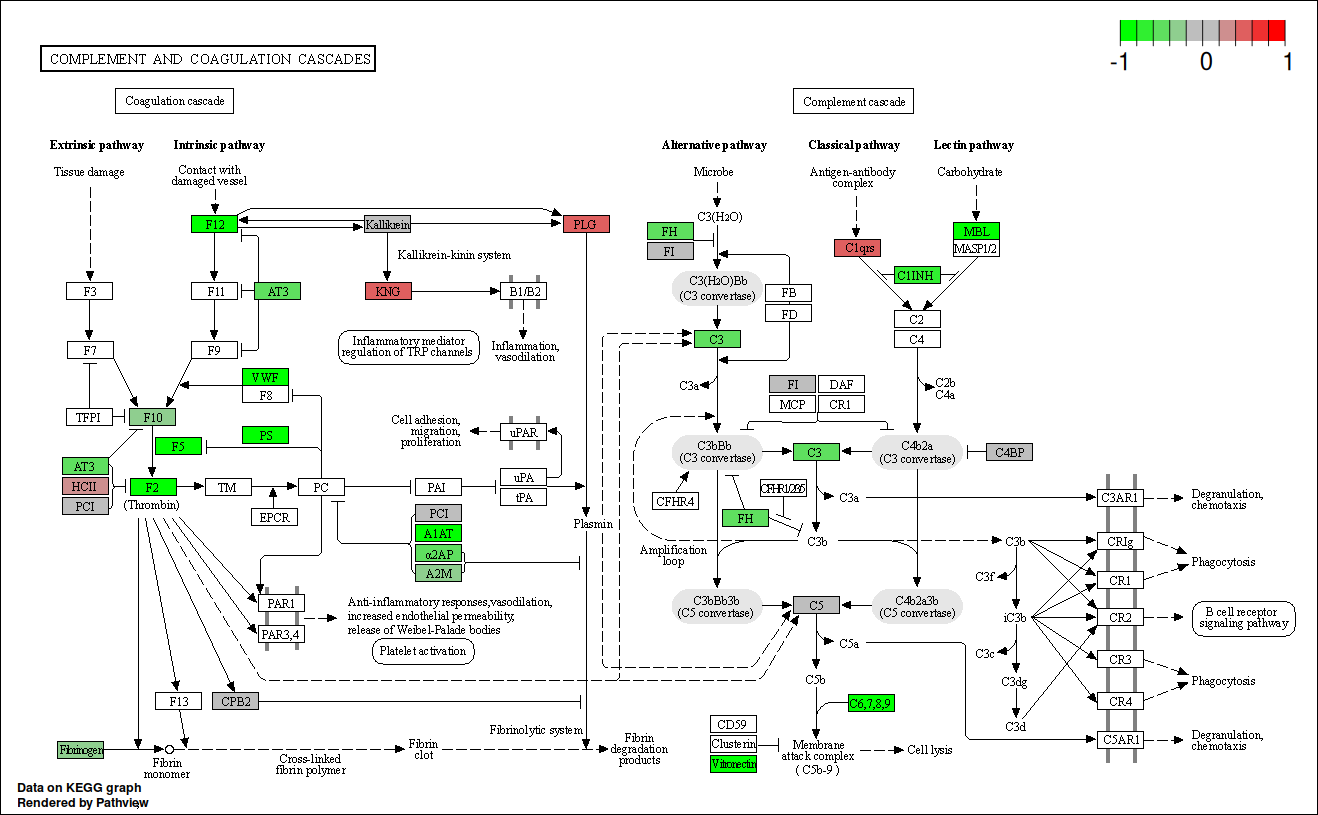
\includegraphics[width=18.31in]{figures/kegg_pathways/hsa04610_pathview} 

}

\caption{KEGG complement cascade pathway annotated with log\(_2\) fold change of proteins in plasma collected 2-weeks post-injury. This compares AIS C SCI patients who experienced an AIS grade improvement and those who did not.}\label{fig:kegg-complement}
\end{figure}

Similarly to the iTRAQ pathway analysis, the label free data analysed via the pathview R package returned the complement and coagulation cascade to be the sole significant KEGG pathway derived from the OpenMS analysed data.
The majority of the proteins present in this pathway were less abundant 2-weeks post-injury in the plasma of AIS C patients who experienced an AIS grade conversion than those who did not (Figure \ref{fig:kegg-complement-chap4}).



\begin{figure}

{\centering 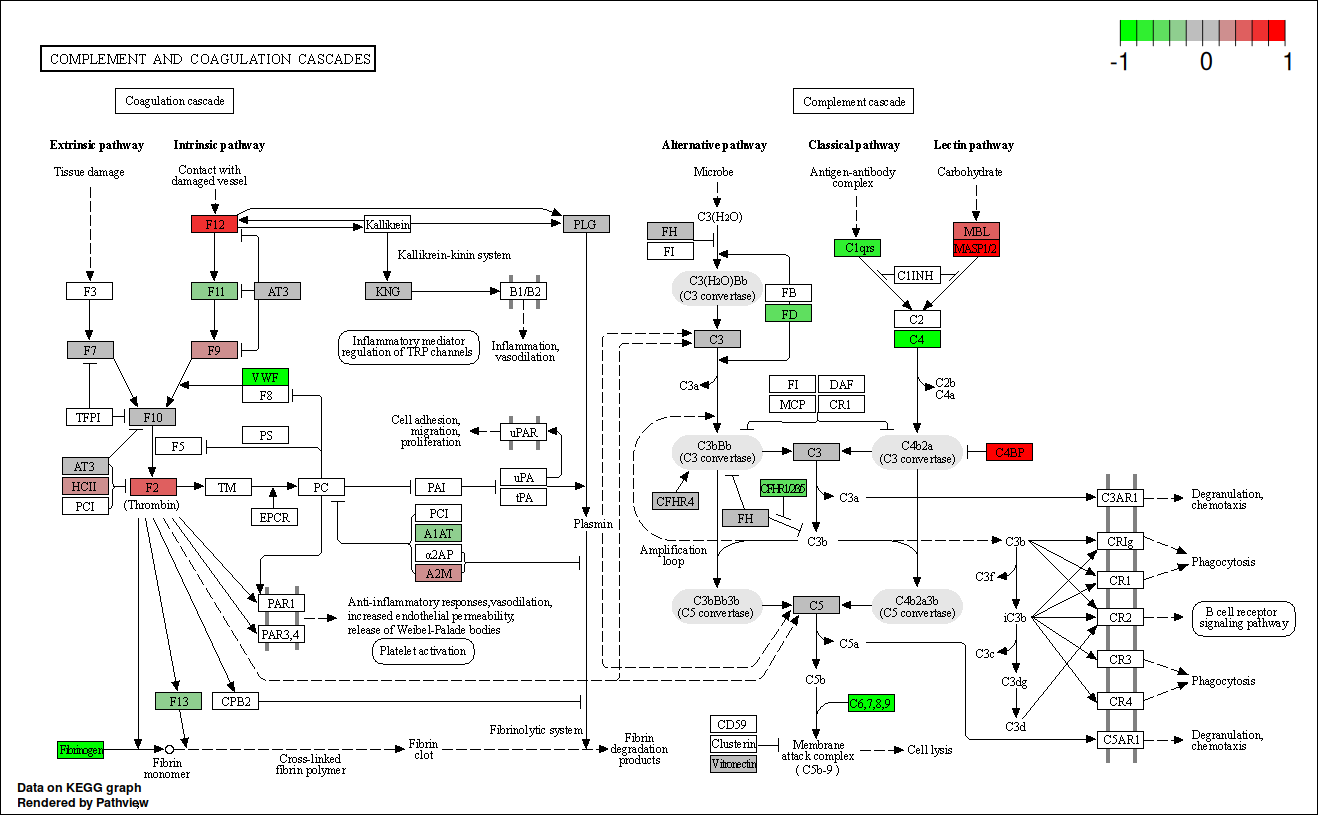
\includegraphics[width=18.31in]{figures/kegg_pathways/hsa04610.pathview_label-free} 

}

\caption{KEGG complement cascade pathway annotated with log\(_2\) fold change of proteins in plasma collected 2-weeks post-injury. This compares AIS C SCI patients who experienced an AIS grade improvement and those who did not.}\label{fig:kegg-complement-chap4}
\end{figure}

\hypertarget{validation-of-proteomic-data-using-elisa}{%
\subsection{Validation of Proteomic Data using ELISA}\label{validation-of-proteomic-data-using-elisa}}

No statistically significant difference between groups for A2M abundance in plasma via DuoSet® ELISAs, though there were outliers in the AIS A and D groups, and particularly in the AIS C patients at 3-months who did not experience an AIS grade conversion (Figure \ref{fig:patchwork-2}).

A significant difference was found between AIS C non-improvers at 2-weeks and AIS D for SAA1, with outliers in AIS C non-improvers at 2-weeks, and both AIS C improvers and non-improvers at 3-months post-injury (Figure \ref{fig:patchwork-2}).
For ApoA1 plasma abundance estimated via Quantikine® ELISAs, statistically significant differences were found between AIS C improvers at 2-weeks and both AIS C improvers and non-improvers at 3-months, AIS C 3-month improvers and AIS A and D, and AIS C 3-month non-improvers and AIS A and D (Figure \ref{fig:patchwork-2}).
A statistically significant difference was also found between AIS C improvers and non-improvers at 2-weeks post-injury for RBP4 (Figure \ref{fig:patchwork-2}).



\begin{figure}
\centering
\includegraphics{proteomic_paper_2020-02-11_files/figure-latex/patchwork-2-1.pdf}
\caption{\label{fig:patchwork-2}Normalised estimated concentration of \(\alpha\)-2-macroglobulin (A), serum amyloid A1 (B), apolipoprotein A1 (C) and retinol binding protein 4 (D). Estimates were calculated from the optical density of a standard curve produced via a DuoSet® ELISA. Plasma from each patient that made up the pooled iTRAQ samples was assayed and pairwise t-tests with bonferroni adjusted P-values were performed to assess differential abundance.}
\end{figure}

\hypertarget{comparing-itraq-and-label-free-proteins}{%
\subsection{Comparing iTRAQ and label-free proteins}\label{comparing-itraq-and-label-free-proteins}}

A total of 87 and 79 unique proteins were identified across the label-free and iTRAQ experiments respectively, with a modest overlap of 26 proteins found using both techniques.



\hypertarget{discussion}{%
\section{Discussion}\label{discussion}}

This is the first study, to our knowledge, to investigate the plasma proteome in SCI patients whose AIS scores either improved or did not improve post injury and also to compare these to AIS grade A and D patients.
We have used two proteomic techniques allowing us to profile both high and low abundance proteins, in order to identify protein candidate biomarkers which may have potential to predict neurological improvement within the acute setting.
Moreover, this data can better inform us of the biology underlying neurological improvement or stability in a cohort of patients being conservatively managed post SCI.

Briefly, for processing of proteomic data, we compared the performance of the mass spectrometry vendor (ABSciex) provided ProteinPilot (version 4.5) and OpenMS (version 2.6.0).
As there were only modest difference in both the proteins identified and the respective fold changes (data not shown), we opted to use OpenMS for the greater transparency and reproducibility it offers as open-source software.

This study has highlighted a number of proteins that may be able to discriminate in, the acute phase following injury, between AIS grade C patients who either improve or do not improve by an AIS grade following SCI.
The most promising of these is Retinol Binding Protein 4 (RBP4) which was demonstrated to be increased in non-improvers compared to improvers in the acute phase.
Further this change could be confirmed using ELISA, which may provide a more clinically useful means of assessment on a wide scale.

RBP4 is synthesised in the liver and binds retinol that is released following vitamin A deficiency.(Peterson 1971)
Once delivered to target cells, retinol can either be converted to retinaldehyde, which is required for functional vision, or oxidised to retinoic acid, which is a ligand for nuclear receptors, thus regulating gene expression.(Lane and Bailey 2005; Balmer and Blomhoff 2002)
The role of retinoid signalling in spinal cord and motor neuron differentiation, including development of regions of the spinal cord has been outlined, and implies a possible involvement in maintaining motor neuron integrity.(Colbert et al. 1995; Sockanathan and Jessell 1998)
The mRNA of a rodent homologue of RBP was found to be up-regulated at 24 hours post-SCI and may promote cell proliferation and regeneration by increasing retinoid metabolism.(Song et al. 2001; Hurst et al. 1999)

Another study of amyotrophic lateral sclerosis (ALS), a neurodegenerative disease, comparing gene expression between post-mortem spinal cord samples of ALS and controls similarly observed up-regulation of RBP1 in ALS spinal cord.(Malaspina, Kaushik, and Belleroche 2001)
Furthermore, a transgenic mouse study reported retinoid signalling may contribute to the retained plasticity and regenerative potential of the mature spinal cord.(Haskell et al. 2002)
Collectively, these results might support a hypothesis that AIS C improvers have increased levels of RBP4 and this relates to improved capacity for neuronal regeneration/plasticity.
Whether this is due to increased expression or due to higher vitamin A dietary intake is unclear from this data.

Alongside RBP4, a number of other protein abundance differences across the different biological comparisons were identified in proteins associated with liver function.
Our previous work investigating the potential of routinely measured haematological analytes for predicting neurological outcome in SCI patients also highlighted several proteins that were linked with liver function; thus providing further support to the theory that liver status is relevant to differential functional recover.(Brown et al. 2019; Bernardo Harrington et al. 2020)
The pathway analysis specifically indicated that the acute phase response (APR) is implicated.

The APR is the bodies first response to infection or injury, including SCI.
This systemic response is largely coordinated by factors released from the liver, but the APRs effects extend to multiple peripheral organs including the kidneys, lungs and spleen.(Bao et al. 2012; Campbell, Zahid, et al. 2008; Fleming et al. 2012; Gris, Hamilton, and Weaver 2008)
This hepatic response is typically transient and quickly fades, but prolonged liver inflammation and pathology has been observed in rodent SCI models.(Goodus et al. 2018; Sauerbeck et al. 2014)
Basic liver functions are chronically impaired by SCI, including metabolising carbohydrates, fats and proteins, storage of minerals vitamins and glycogen and filtering blood from the digestive tract.(García-López et al. 2007; DeLeve 2007; Farkas and Gater 2018; Chow et al. 2012; Sauerbeck et al. 2014)

The acute (1-7 days) liver response to SCI is well documented; the inflammatory cytokines including TNF\(\alpha\), IL-1\(\alpha\), IL-1\(\beta\) and IL-6, released at the injury site, reach the liver through the bloodstream.(Fleming et al. 2012; Hundt et al. 2011)
This provokes the liver to enter the APR and produce acute phase proteins thus stimulating a greater immune response.(Anthony and Couch 2014; Fleming et al. 2012)
The hepatocytes that make up the majority of the liver biomass, express receptors that bind the aforementioned inflammatory cytokines; similarly the hepatic macrophage Kupffer cells also bind these cytokines, complement proteins and lipopolysaccharide (LPS) and swiftly remove microorganisms, endotoxins and other debris from the blood.(Yang et al. 2013; Szalai et al. 2000; Crispe 2016; Campbell et al. 2005)
Furthermore, it has been suggested that liver inflammation and Kupffer cells activity promote recruitment of leukocytes to the injury site in brain or spinal trauma, potentially enhancing CNS injury.(Anthony and Couch 2014; Campbell et al. 2005)
For example, a rodent study demonstrated depletion of Kupffer cells prior to injury resulted in few neutrophils infiltrating the injury site.(Campbell, Zahid, et al. 2008; Campbell, Anthony, et al. 2008)

Another protein that out label-free proteomic data highlights is Peroxiredoxin 2 (PRX-2), which was detected acutely in AIS C improvers and AIS D patients, and subacutely in AIS A and AIS D. Peroxiredoxins are a large and highly conserved family of enzymes that reduce peroxides.
PRX-2 is highly abundant in RBCs and intracellularly serves as an important anti-oxidant role in various cells types, including neurons.(Low, Hampton, and Winterbourn 2008)
By contrast, extracellular PRX-2 has been suggested to act as an inflammatory DAMP, leading microglia and macrophages to release a plethora of pro-inflammatory factors.(Salzano et al. 2014; Garcia-Bonilla and Iadecola 2012; Shichita et al. 2012)
An \emph{in vitro} primary neurons and microglia co-culture study reported PRX-2 activating microglia via TLR-4, potentially leading to neuronal apoptosis.(Lu et al. 2018)
A murine study found over-expression of PRX-2 attenuated oxidative stress and neuronal apoptosis following subarachnoid haemorrhage.(Lu et al. 2019)
Over-expression of PRX-2 is speculated to protect again ischaemic neuronal injury by modulating the redox-sensitive thioredoxin-apoptosis signal-regulating kinase (ASK) 1 signalling complex.(Gan et al. 2012)
Several molecular chaperones can interact with ASK1, including thioredoxin and TNF receptor-associated factor 6.(Matsuzawa et al. 2005)
The dissociation of the thioredoxin-ASK1 complex activates ASK1.
PRX-2 is oxidised after scavenging free radicals, whereupon its antioxidantive activity is reduced.
This inactivation can be reversed by the thioredoxin-thioredoxin reductase system, whereby oxidised PRX-2 can regain its activity by reducing thioredoxin, leading to the dissociation of the thioredoxin-ASK1 complex.(Rhee and Woo 2011)
Additionally, oxidised PRX-1 can inhibit ASK1-induced apoptosis via the thioredoxin-binding domain on ASK1.(Kim, Kim, and Lee 2008)

The presence of PRX-2 in acute AIS C improvers and absence in acute C non-improvers suggests the protein could indicate a more protective action against oxidative stress, and implies the protein has potential value as a biomarker of functional outcomes.
Similarly, PRX-2 may be acting as a healthy response to trauma-induced oxidative stress in both acute AIS D, although the persistence to the subacute time-point is less clear.
Likewise, the presence of PRX-2 in AIS A subacutely, but not acutely is more perplexing.
It should be noted that as plasma was used and cells were lysed, there is no distinction between intracellular and extracellular PRX-2 in this data.
Perhaps in the more severe AIS A injury, secondary injuries, including oxidative stress, are greater and so persist to the subacute time-point.
The acute absence may be a result of an overwhelmed physiology unable to respond or prioritise managing oxidative stress.

Pathway analysis from both the iTRAQ and label-free experiments identified the complement and coagulation cascades as a significant pathway of interest.
More broadly, the trend in this data is for proteins in the complement pathway is lower abundance, or inhibitory proteins such as C4BP to be more abundant, in the acute improvers.
C3 for instance, cleavage of which is vital for complement activation, was less abundant in acute AIS C improvers relative to non-improvers.
This finding is in line with a genetic C3 knockout study in mice which reported better neurological scores 2 days post-injury, reduced residual consolidated neurological deficit at 21 days and display minor change in reduced gliosis (20\% decrease at 1h timepoint) but a three-to-fourfold decrease in neutrophil infiltration, resulting in enhanced regeneration of axons.(Qiao et al. 2006)
Another study using a similar C3 knockout model reported improved neurological scores at acute and long-term time points.(Guo et al. 2010)
These results imply that the complement cascade is a particularly important component of a differential response to neurological injury which ultimately leads to greater functional recovery.
Given the complexity of the complement cascade and the limited time points in this study, further work is needed to elucidate which facets of the cascade are outcome modifying, and at which stages post-injury.

AIS A and D samples were included largely to compare to the AIS C improvers.
If the improvers were all just a less severe AIS C, we might expect them to be more similar to the AIS D samples, with the non-improvers being closer to the As.
As this is not what we observed, we can conclude there is more to the differential functional recovery than initial injury severity.

The small number of statistically significant proteins speaks to the variability of human plasma samples, and is likely exacerbated by the inconstant timing of sample collection relative to injury.
Thus, a repeat of this experiment with a larger sample size will likely reveal many more proteins of potential interest.
Regardless, this study has highlighted RPB4 and PRX-2 as potential biomarkers of functional recover.
We have also highlighted the complement cascade as being a particularly important pathway in differential recovery.
Additional investigation of these proteins, but also the complement cascade more broadly, particularly at more acute time points, would also be valuable.
Furthermore, a metabolomic analysis with a similar samples would greatly compliment this work, particularly with regards to investigating further links to the livers role in neurological recovery.
Similarly, this additional work could complement the AIS A and D sample data, which may reveal further insights from this data.

\newpage

\hypertarget{sup-data}{%
\section*{Supplementary material}\label{sup-data}}
\addcontentsline{toc}{section}{Supplementary material}

\beginsupplement

\hypertarget{session-information}{%
\subsection{Session Information}\label{session-information}}

\begin{verbatim}
##                _                           
## platform       aarch64-apple-darwin20      
## arch           aarch64                     
## os             darwin20                    
## system         aarch64, darwin20           
## status                                     
## major          4                           
## minor          1.3                         
## year           2022                        
## month          03                          
## day            10                          
## svn rev        81868                       
## language       R                           
## version.string R version 4.1.3 (2022-03-10)
## nickname       One Push-Up
\end{verbatim}

\clearpage

\begin{table}

\caption{\label{tab:package-table}Packages Used}
\centering
\begin{tabular}[t]{lll}
\toprule
package & version & date\\
\midrule
base & 4.1.3 & 2022-03-18\\
MSstats & 4.2.0 & 2021-05-31\\
STRINGdb & 2.6.5 & 2020-01-10\\
ReactomePA & 1.38.0 & 2021-10-26\\
rlang & 1.0.3 & 2022-06-27\\
\addlinespace
bookdown & 0.27 & 2022-06-14\\
lime & 0.5.2 & 2021-02-24\\
RColorBrewer & 1.1.3 & 2022-04-03\\
ggVennDiagram & 1.2.0 & 2021-10-19\\
DiagrammeR & 1.0.9 & 2022-03-04\\
\addlinespace
patchwork & 1.1.1 & 2020-12-15\\
cowplot & 1.1.1 & 2020-12-15\\
BiocManager & 1.30.18 & 2022-05-18\\
knitr & 1.39 & 2022-04-26\\
naniar & 0.6.1 & 2021-05-14\\
\addlinespace
psych & 2.2.5 & 2022-05-01\\
Hmisc & 4.7.0 & 2022-04-12\\
Formula & 1.2.4 & 2020-10-16\\
survival & 3.3.1 & 2022-02-20\\
lattice & 0.20.45 & 2021-09-18\\
\addlinespace
bibtex & 0.4.2.3 & 2020-09-19\\
captioner & 2.2.3 & 2015-07-15\\
kableExtra & 1.3.4 & 2021-02-19\\
rmarkdown & 2.14 & 2022-04-25\\
minpack.lm & 1.2.2 & 2022-04-13\\
\addlinespace
MASS & 7.3.57 & 2022-04-05\\
data.table & 1.14.2 & 2021-09-23\\
lubridate & 1.8.0 & 2021-10-03\\
janitor & 2.1.0 & 2021-01-04\\
RPostgreSQL & 0.7.3 & 2021-10-22\\
\addlinespace
DBI & 1.1.3 & 2022-06-18\\
readxl & 1.4.0 & 2022-03-28\\
forcats & 0.5.1 & 2021-01-27\\
stringr & 1.4.0 & 2019-02-09\\
dplyr & 1.0.9 & 2022-04-27\\
\addlinespace
purrr & 0.3.4 & 2020-04-16\\
readr & 2.1.2 & 2022-01-30\\
tidyr & 1.2.0 & 2022-01-27\\
tibble & 3.1.7 & 2022-04-26\\
ggplot2 & 3.3.6 & 2022-04-27\\
\addlinespace
tidyverse & 1.3.1 & 2021-04-15\\
\bottomrule
\end{tabular}
\end{table}

\clearpage

\begin{landscape}\begingroup\fontsize{5}{7}\selectfont

\begin{longtable}[t]{>{\raggedright\arraybackslash}p{0.5cm}>{\raggedleft\arraybackslash}p{1.6cm}>{\raggedleft\arraybackslash}p{1.6cm}>{\raggedleft\arraybackslash}p{1.6cm}>{\raggedleft\arraybackslash}p{1.6cm}>{\raggedleft\arraybackslash}p{1.6cm}>{\raggedleft\arraybackslash}p{1.6cm}>{\raggedleft\arraybackslash}p{1.6cm}>{\raggedleft\arraybackslash}p{1.6cm}>{\raggedleft\arraybackslash}p{1.6cm}>{\raggedleft\arraybackslash}p{1.6cm}}
\caption{\label{tab:openms-fc-table}OpenMS log$_2$ fold changes in the plasma proteome of SCI patients from iTRAQ experiments. 'Acute' and 'Subacute' samples collected within 2 week and approximately 3-months post-injury respectively.}\\
\toprule
gene & Acute AIS C improvers vs non-improvers & Subacute AIS C improvers vs non-improvers & AIS C improvers acute vs subacute & AIS C non-improvers acute vs subacute & AIS C improvers vs non-improvers & AIS A vs D & AIS C improvers vs A & AIS C improvers vs D & AIS C non-improvers vs A & AIS C non-improvers vs D\\
\midrule
\endfirsthead
\caption[]{\label{tab:openms-fc-table}OpenMS log$_2$ fold changes in the plasma proteome of SCI patients from iTRAQ experiments. 'Acute' and 'Subacute' samples collected within 2 week and approximately 3-months post-injury respectively. \textit{(continued)}}\\
\toprule
gene & Acute AIS C improvers vs non-improvers & Subacute AIS C improvers vs non-improvers & AIS C improvers acute vs subacute & AIS C non-improvers acute vs subacute & AIS C improvers vs non-improvers & AIS A vs D & AIS C improvers vs A & AIS C improvers vs D & AIS C non-improvers vs A & AIS C non-improvers vs D\\
\midrule
\endhead

\endfoot
\bottomrule
\endlastfoot
A1BG & -0.9032 & -0.1018 & -0.6088 & 0.1926 & 0.2253 & 0.7937 & -0.3498 & 0.4440 & -0.5750 & 0.2187\\
A2M & -1.0386 & -0.2464 & -0.6761 & 0.1161 & -1.2301 & 1.4248 & -1.6030 & -0.1782 & -0.3729 & 1.0519\\
AFM & -0.3788 & -1.2249 & 0.4815 & -0.3645 & 0.5518 & 1.1924 & -1.2566 & -0.0642 & -1.8084 & -0.6160\\
AHSG & 1.1795 &  & -0.5545 &  &  &  &  &  &  & \\
AMBP & 0.6562 & -0.3433 & 0.8607 & -0.1389 & -0.9023 &  & 1.2038 &  & 2.1061 & \\
\addlinespace
APCS & 0.1498 & 0.2109 & -0.0114 & 0.0497 &  & 0.3557 &  &  & -0.0495 & 0.3063\\
APOA1 & -0.1817 & -0.6924 & -0.2338 & -0.7444 & -0.7677 & 0.6941 & -1.3173 & -0.6232 & -0.5496 & 0.1446\\
APOA2 & 0.0900 & -1.1461 & -0.6668 & -1.9029 &  &  &  &  &  & \\
APOA4 & 0.1296 & 0.9637 & -1.2313 & -0.3972 & -1.3254 & 0.7876 & -1.3347 & -0.5471 & -0.0093 & 0.7783\\
APOB & 0.1379 & -0.0164 & -0.6333 & -0.7876 & -0.8570 & 0.5260 & -1.2346 & -0.7086 & -0.3775 & 0.1485\\
\addlinespace
APOE & -1.2134 & 0.2931 & -0.6884 & 0.8180 & -0.9078 & 0.7747 & -1.5477 & -0.7731 & -0.6399 & 0.1347\\
APOH & -0.3602 & -0.7025 & -0.6445 & -0.9867 & -0.9997 & 2.8144 & -1.0092 & 1.8052 & -0.0095 & 2.8048\\
APOL1 & -1.1791 & -0.5194 & -1.0440 & -0.3843 & -0.1153 & 0.5653 & 0.1299 & 0.6952 & 0.2452 & 0.8105\\
APOM & -1.2168 & -0.6820 & 0.6935 & 1.2283 &  & 0.6562 &  &  & 0.6665 & 1.3227\\
ATRN &  &  & -1.0063 &  &  &  &  &  &  & \\
\addlinespace
AZGP1 & 1.2192 & 1.0252 & 0.0811 & -0.1129 & -3.3890 & -3.6441 & 0.3703 & -3.2738 & 3.7592 & 0.1152\\
C1QB & -0.8410 & -2.0020 & 0.7071 & -0.4539 & -1.9729 & 1.3563 & -2.0066 & -0.6503 & -0.0337 & 1.3226\\
C1R & -0.4335 & -0.7632 & 0.0366 & -0.2931 & -0.1467 & 0.7976 & 0.3564 & 1.1540 & 0.5032 & 1.3008\\
C1S & 0.0295 & -0.8194 & 0.1680 & -0.6809 &  &  &  &  &  & \\
C2 &  &  &  &  & -2.5581 & 2.5641 & -2.5953 & -0.0312 & -0.0372 & 2.5269\\
\addlinespace
C3 & -0.7441 & -0.6969 & 0.0652 & 0.1124 & -1.0731 & 1.2388 & -2.1616 & -0.9228 & -1.0886 & 0.1503\\
C4BPA & -0.1810 & -2.4455 & 1.6628 & -0.6017 & -1.2379 & 1.5490 & -1.8449 & -0.2959 & -0.6070 & 0.9420\\
C5 & -0.5448 & -0.2031 & 0.9230 & 1.2647 & -0.7200 & 1.2710 & -1.6769 & -0.4058 & -0.9569 & 0.3142\\
C6 & -1.3936 & 1.7817 & -1.3097 & 1.8656 & -3.0452 & 1.7642 & -3.2550 & -1.4908 & -0.2098 & 1.5544\\
C7 & -0.9642 & 0.8848 & -0.7827 & 1.0663 & 0.9970 & 0.0709 & -1.1136 & -1.0428 & -2.1107 & -2.0398\\
\addlinespace
C8A & -0.5118 & 0.2737 & -0.7630 & 0.0224 & -2.8108 & 0.1731 & -2.1285 & -1.9554 & 0.6823 & 0.8554\\
C8B & -2.1950 & 0.2789 & -1.5955 & 0.8785 & -1.8944 & -0.4803 & -0.9598 & -1.4400 & 0.9346 & 0.4544\\
C8G &  &  & -1.6305 &  &  &  &  &  &  & \\
C9 & -2.2199 & 0.4534 & -1.9250 & 0.7483 & -0.7346 & 0.6496 & -3.2424 & -2.5928 & -2.5078 & -1.8583\\
CD5L & -0.9293 & -0.6205 & -0.7146 & -0.4057 & -2.4643 & 0.4483 & -2.3260 & -1.8778 & 0.1383 & 0.5865\\
\addlinespace
CFH & -1.1240 & 0.7407 & -1.6481 & 0.2166 & -1.0359 & 0.1380 & -1.3260 & -1.1880 & -0.2902 & -0.1522\\
CFI &  & 0.5360 &  & 1.2578 &  &  &  &  &  & \\
CLU & -1.1959 & -0.8682 & -0.1722 & 0.1555 & -1.3664 & 0.8252 & -2.1976 & -1.3724 & -0.8312 & -0.0060\\
CP & -0.3892 & 0.2565 & -0.4537 & 0.1920 & -0.6658 & 0.4235 & -0.2696 & 0.1540 & 0.3962 & 0.8197\\
F12 & 0.4852 & -0.9398 & 0.6703 & -0.7547 & -0.8534 & 0.5550 & -1.3146 & -0.7596 & -0.4612 & 0.0938\\
\addlinespace
F2 & -0.7493 & -0.7564 & 0.0983 & 0.0912 & -0.5409 & 1.1677 & -1.5476 & -0.3799 & -1.0067 & 0.1610\\
FCN3 &  & 0.9645 &  &  &  &  &  &  &  & \\
FGA & -0.9591 & -0.5109 & 0.4842 & 0.9324 & -1.0156 & 1.0487 & -1.4708 & -0.4221 & -0.4552 & 0.5934\\
FGB & -0.8339 & -0.1254 & 0.0684 & 0.7770 & -0.8343 & 1.0951 & -1.4647 & -0.3695 & -0.6303 & 0.4648\\
FGG & -1.1433 & -0.0247 & -0.2978 & 0.8208 & -0.7191 & 0.7607 & -1.0780 & -0.3173 & -0.3589 & 0.4018\\
\addlinespace
FN1 & -0.2796 & -0.3153 & 0.2899 & 0.2541 & -0.5778 & 1.1463 & -1.2551 & -0.1088 & -0.6773 & 0.4690\\
GC & -0.5583 & 0.4051 & -0.7950 & 0.1684 & -1.8700 & -0.2961 & -1.2641 & -1.5602 & 0.6059 & 0.3098\\
GSN & 0.0705 & 0.0479 & -0.6710 & -0.6935 &  &  &  &  &  & \\
HABP2 &  &  &  &  & -0.5367 & 1.4446 & -0.7071 & 0.7375 & -0.1704 & 1.2742\\
HP & -1.2469 & 0.5276 & -0.3488 & 1.4257 & -0.6394 & 0.9683 & -1.2963 & -0.3280 & -0.6570 & 0.3114\\
\addlinespace
HPX & -0.4105 & -0.2881 & -0.7115 & -0.5891 & -0.3598 & 0.9360 & -1.1034 & -0.1674 & -0.7437 & 0.1924\\
HRG & 0.5979 & 1.0673 & 0.0322 & 0.5015 & -0.7301 & 0.6894 & -0.8232 & -0.1338 & -0.0931 & 0.5963\\
IGHA1 & 1.7636 & 1.3477 & 0.3629 & -0.0530 & -2.0152 & 0.4328 & -2.2081 & -1.7753 & -0.1929 & 0.2399\\
IGHD &  &  &  &  & -2.4500 & 0.4182 & -3.4285 & -3.0102 & -0.9785 & -0.5603\\
IGHG1 & -0.0855 & 0.9292 & -0.4963 & 0.5184 & -0.0970 & -1.8091 & 0.4814 & -1.3277 & 0.5785 & -1.2306\\
\addlinespace
IGHG2 & 0.9720 & 0.3502 & 0.4608 & -0.1611 & -0.6249 & -1.5107 & 0.2705 & -1.2401 & 0.8955 & -0.6152\\
IGHG3 & -0.1942 & 1.4323 & -0.9310 & 0.6955 & -1.8544 & -0.3927 & -1.8870 & -2.2798 & -0.0327 & -0.4254\\
IGHM & -0.6318 & -0.8967 & -0.4175 & -0.6824 & -1.1742 & 1.7916 & -2.3509 & -0.5593 & -1.1767 & 0.6149\\
IGKC & -0.0697 & 0.0420 & -0.1150 & -0.0032 & -1.1868 & -0.2875 & -1.1765 & -1.4641 & 0.0103 & -0.2772\\
IGKV3D-20 &  &  &  &  & -0.3699 & -0.0537 & 0.2115 & 0.1578 & 0.5814 & 0.5277\\
\addlinespace
ITIH1 & -0.9767 & 0.7057 & -0.5212 & 1.1612 & -0.6149 & 0.5496 & -0.5039 & 0.0456 & 0.1110 & 0.6605\\
ITIH2 & -0.3143 & -0.5283 & -0.2363 & -0.4504 & -0.7432 & 0.6757 & -1.2137 & -0.5379 & -0.4705 & 0.2052\\
ITIH3 & -0.5456 & 0.6139 & 0.3513 & 1.5108 & -2.0564 & 1.2902 & -1.8743 & -0.5841 & 0.1821 & 1.4724\\
ITIH4 & -0.0670 & -0.2189 & 0.3809 & 0.2289 & -1.0844 & 0.9773 & -1.8198 & -0.8425 & -0.7355 & 0.2418\\
KLKB1 &  & -2.2093 &  & -0.2714 &  &  &  &  &  & \\
\addlinespace
KNG1 & -0.6198 & -0.0025 & -0.0676 & 0.5497 & -0.6644 & 0.8053 & 0.0312 & 0.8365 & 0.6956 & 1.5009\\
LRG1 & -0.7988 & 0.2565 & 0.1402 & 1.1955 & -0.9516 & 1.7018 & -2.1951 & -0.4933 & -1.2435 & 0.4583\\
LUM & 0.0832 & 0.6580 & -1.2636 & -0.6888 &  &  &  &  &  & \\
ORM1 & -0.1975 & 1.1178 & -0.2240 & 1.0913 & -1.9126 & 1.6761 & -1.3026 & 0.3735 & 0.6100 & 2.2862\\
PGLYRP2 &  &  &  &  &  &  &  &  &  & \\
\addlinespace
PLG & -0.3680 & 0.0881 & -0.8410 & -0.3850 & -1.0702 & 2.7112 & -2.8493 & -0.1381 & -1.7792 & 0.9321\\
PROS1 & -0.3301 & 0.0624 & -0.7963 & -0.4039 & -0.5090 & 1.5350 & -3.8745 & -2.3396 & -3.3656 & -1.8306\\
RBP4 & 0.4506 & 0.4186 & -0.0212 & -0.0532 & -4.0971 & 1.4352 & -2.9877 & -1.5525 & 1.1094 & 2.5446\\
SAA1 & -2.7778 & 2.3464 & -0.5152 & 4.6090 & -1.3859 & 2.4855 & -2.5594 & -0.0739 & -1.1735 & 1.3120\\
SERPINA1 & 0.6826 & 0.0482 & 1.7824 & 1.1481 & -0.0999 & -0.1559 & -1.3635 & -1.5194 & -1.2636 & -1.4195\\
\addlinespace
SERPINA3 & -0.7582 & -0.1618 & 0.1837 & 0.7802 & -0.7418 & 2.2311 & -2.0353 & 0.1958 & -1.2936 & 0.9375\\
SERPINA4 & 0.0099 &  & -1.0180 &  & -1.4474 &  & -0.6572 &  & 0.7902 & \\
SERPINA5 &  &  &  & 0.2757 &  &  &  &  &  & \\
SERPINC1 & -0.5553 & -0.2339 & -0.5421 & -0.2207 & -0.7720 & 1.1067 & -1.3465 & -0.2398 & -0.5744 & 0.5322\\
SERPIND1 & 0.2536 &  & 0.0459 &  & 0.3050 & 2.3844 & -1.6469 & 0.7375 & -1.9519 & 0.4325\\
\addlinespace
SERPING1 & -1.1615 & 0.1192 & -1.3511 & -0.0705 & -0.9302 & 1.0767 & -1.0905 & -0.0138 & -0.1603 & 0.9164\\
TF & -0.2824 & -0.1105 & -0.4844 & -0.3125 & -0.7682 & 0.5876 & -0.9946 & -0.4070 & -0.2264 & 0.3612\\
VTN & -0.6186 & -0.0324 & -0.2690 & 0.3172 & -1.7235 & 1.4919 & -2.1518 & -0.6599 & -0.4283 & 1.0636\\
VWF &  & 1.0586 &  & 1.3918 & -2.5663 & 0.5162 & -1.9774 & -1.4612 & 0.5889 & 1.1051\\*
\end{longtable}
\endgroup{}
\end{landscape}

\begin{landscape}\begingroup\fontsize{5}{7}\selectfont

\begin{longtable}[t]{>{\raggedright\arraybackslash}p{0.5cm}>{\raggedleft\arraybackslash}p{1.6cm}>{\raggedleft\arraybackslash}p{1.6cm}>{\raggedleft\arraybackslash}p{1.6cm}>{\raggedleft\arraybackslash}p{1.6cm}>{\raggedleft\arraybackslash}p{1.6cm}>{\raggedleft\arraybackslash}p{1.6cm}>{\raggedleft\arraybackslash}p{1.6cm}>{\raggedleft\arraybackslash}p{1.6cm}>{\raggedleft\arraybackslash}p{1.6cm}}
\caption{\label{tab:label-free-fc-table1}OpenMS log$_2$ fold changes in the plasma proteome of SCI patients from label-free experiments. 'Acute' and 'Subacute' samples collected within 2 week and approximately 3-months post-injury respectively.}\\
\toprule
Protein & Acute A Vs Subacute D & Acute C Improvers Vs Subacute D & Acute C Improvers Vs Subacute A & Acute C Non-Improvers Vs Subacute A & Acute A Vs Acute C Improvers & Acute A Vs Subacute C Non-Improvers & Acute A Vs Subacute A & Acute A Vs Subacute C Improvers & Acute C Non-Improvers Vs Subacute D\\
\midrule
\endfirsthead
\caption[]{\label{tab:label-free-fc-table1}OpenMS log$_2$ fold changes in the plasma proteome of SCI patients from label-free experiments. 'Acute' and 'Subacute' samples collected within 2 week and approximately 3-months post-injury respectively. \textit{(continued)}}\\
\toprule
Protein & Acute A Vs Subacute D & Acute C Improvers Vs Subacute D & Acute C Improvers Vs Subacute A & Acute C Non-Improvers Vs Subacute A & Acute A Vs Acute C Improvers & Acute A Vs Subacute C Non-Improvers & Acute A Vs Subacute A & Acute A Vs Subacute C Improvers & Acute C Non-Improvers Vs Subacute D\\
\midrule
\endhead

\endfoot
\bottomrule
\endlastfoot
AFM &  & -0.7786 &  & -1.1371 &  &  &  &  & -1.3604\\
AHSG &  & -2.7643 & -3.4309 & -3.3017 &  &  & -1.9761 &  & \\
APOA4 & -1.0588 &  &  &  &  & -1.2657 &  & -1.1544 & \\
APOC3 &  &  &  &  & -1.4275 & -1.6878 &  &  & \\
APOH &  & -1.3700 &  &  &  &  &  &  & -1.5614\\
\addlinespace
APOL1 &  &  &  &  &  &  & -0.8923 &  & \\
AQR &  &  &  &  &  &  &  & 0.6965 & \\
C4BPA &  & 1.2058 &  &  &  &  &  &  & \\
C4BPB &  & 1.3009 &  &  &  &  &  & 1.3841 & \\
C8G &  & -1.2253 & -1.0543 &  & 1.1118 &  &  &  & \\
\addlinespace
C9 & 1.4444 & 1.0533 &  &  &  & 1.0217 &  & 1.2553 & 1.3765\\
CFH & 0.5112 & 0.5790 &  &  &  &  &  &  & \\
CFHR1 &  & 0.9812 &  &  &  &  &  & 1.4700 & \\
CFHR5 & 1.3097 &  &  &  &  &  &  &  & \\
CLEC3B & -1.9123 & -1.5100 &  &  &  & -1.4447 &  & -1.3585 & -1.6640\\
\addlinespace
COMP &  & -2.2269 & -2.8311 & -2.3546 &  &  & -2.4495 &  & \\
CRP & 4.0520 &  &  &  &  & 3.8525 &  &  & 3.3381\\
ECM1 &  & -1.8865 &  &  &  &  &  &  & \\
F10 &  & 1.1353 &  &  &  &  &  &  & \\
F13A1 & -2.0331 & -1.9770 & -1.9454 &  &  & -1.8768 & -2.0015 & -2.0606 & \\
\addlinespace
F2 &  & 1.0044 & 0.8140 &  &  &  &  &  & \\
F7 &  &  &  &  & -0.7634 &  &  &  & \\
F9 &  & 1.0227 &  &  &  &  &  &  & \\
FCN3 &  &  &  &  &  & -1.1449 &  & -0.9483 & \\
FGA & 1.0806 & 0.7180 &  &  &  & 1.0275 &  & 0.7479 & 1.0928\\
\addlinespace
FGB & 0.7119 & 0.5186 &  & 0.7340 &  & 0.7738 &  & 0.5500 & 0.9761\\
FGL1 & 2.5544 &  &  &  &  & 2.5246 &  & 2.4956 & \\
GPLD1 &  &  &  &  & -1.4430 &  &  &  & \\
GPX3 & 0.8877 & 0.7335 &  &  &  &  &  &  & \\
HABP2 & 0.9940 & 1.1355 &  &  &  &  &  &  & \\
\addlinespace
HRG & -0.6336 &  &  &  &  &  &  &  & \\
HYI &  &  &  &  &  &  & -1.0768 &  & \\
IGHG2 &  & -1.8011 &  &  &  &  &  &  & \\
IGHG4 &  &  & -2.2253 & -2.6735 &  &  &  &  & \\
IGLV3-19 &  &  & -1.9672 &  &  &  &  &  & \\
\addlinespace
ITIH1 &  &  &  &  &  & -1.0172 &  &  & \\
ITIH4 & 1.9473 & 3.9089 & 0.8010 & 0.8216 &  &  & 0.8095 & 1.3021 & 1.4555\\
LBP & 2.0666 &  &  &  &  & 1.6765 & 1.7122 & 1.8745 & 1.6204\\
LGALS3BP &  &  & 1.9633 &  &  &  &  &  & \\
LUM & -1.3539 & -1.2002 & -1.2800 & -1.4246 &  & -1.6006 & -1.4338 & -1.1914 & -1.3447\\
\addlinespace
LYZ &  &  &  & 1.2935 &  &  &  &  & \\
MASP1 &  & 0.9681 &  &  & -1.0112 &  &  &  & \\
MASP2 &  & 0.9549 & 0.9501 &  &  &  &  &  & \\
ORM1 &  & -1.2827 &  &  & 1.2451 &  &  &  & \\
PCOLCE & -1.9201 &  &  &  & -1.7506 &  &  &  & \\
\addlinespace
PGLYRP2 & -1.2799 & -0.9299 & -1.1251 & -1.4588 &  & -1.4051 & -1.4751 & -1.2655 & -1.2637\\
PLG &  & 0.3879 &  &  &  &  &  & 0.3532 & \\
PRG4 & 1.8915 & 1.9399 & 1.7628 &  &  & 1.4891 & 1.7144 & 1.3478 & \\
RNASE4 &  &  & 4.3884 &  &  &  & 3.9924 &  & \\
SAA1 & 5.4086 &  &  &  &  & 4.5431 &  & 3.6939 & 4.3015\\
\addlinespace
SAA2 &  &  &  &  & 4.4465 &  &  &  & \\
SERPINA10 &  & 0.9102 &  &  &  &  &  &  & \\
SERPINA4 & -1.8496 & -1.2216 &  & -1.3820 &  & -1.9414 & -1.5613 & -1.3615 & -1.6703\\
SERPINF1 & -1.1883 &  &  &  &  &  &  &  & \\
THBS1 &  &  & 2.8162 &  &  &  &  &  & \\
\addlinespace
Trypsin &  & -0.5747 &  &  &  &  &  &  & \\
VTN &  & 0.7175 & 0.6959 &  &  &  &  & 0.7629 & \\*
\end{longtable}
\endgroup{}
\end{landscape}

\begin{landscape}\begingroup\fontsize{5}{7}\selectfont

\begin{longtable}[t]{>{\raggedright\arraybackslash}p{0.5cm}>{\raggedleft\arraybackslash}p{1.6cm}>{\raggedleft\arraybackslash}p{1.6cm}>{\raggedleft\arraybackslash}p{1.6cm}>{\raggedleft\arraybackslash}p{1.6cm}>{\raggedleft\arraybackslash}p{1.6cm}>{\raggedleft\arraybackslash}p{1.6cm}>{\raggedleft\arraybackslash}p{1.6cm}>{\raggedleft\arraybackslash}p{1.6cm}>{\raggedleft\arraybackslash}p{1.6cm}}
\caption{\label{tab:label-free-fc-table2}OpenMS log$_2$ fold changes in the plasma proteome of SCI patients from label-free experiments. 'Acute' and 'Subacute' samples collected within 2 week and approximately 3-months post-injury respectively.}\\
\toprule
Protein & Acute D Vs Subacute A & Acute C Improvers Vs Subacute C Improvers & Acute C Non-Improvers Vs Subacute C Non-Improvers & Acute C Non-Improvers Vs Subacute C Improvers & Acute D Vs Subacute D & Acute A Vs Acute D & Acute C Improvers Vs Subacute C Non-Improvers & Acute D Vs Subacute C Improvers & Acute D Vs Subacute C Non-Improvers\\
\midrule
\endfirsthead
\caption[]{\label{tab:label-free-fc-table2}OpenMS log$_2$ fold changes in the plasma proteome of SCI patients from label-free experiments. 'Acute' and 'Subacute' samples collected within 2 week and approximately 3-months post-injury respectively. \textit{(continued)}}\\
\toprule
Protein & Acute D Vs Subacute A & Acute C Improvers Vs Subacute C Improvers & Acute C Non-Improvers Vs Subacute C Non-Improvers & Acute C Non-Improvers Vs Subacute C Improvers & Acute D Vs Subacute D & Acute A Vs Acute D & Acute C Improvers Vs Subacute C Non-Improvers & Acute D Vs Subacute C Improvers & Acute D Vs Subacute C Non-Improvers\\
\midrule
\endhead

\endfoot
\bottomrule
\endlastfoot
AFM &  &  & -1.216 & -1.0952 &  &  &  &  & \\
AHSG & -2.441 &  &  &  &  &  &  &  & \\
APOH &  &  &  &  & -1.754 &  &  &  & \\
C1QA &  &  &  & 1.4061 &  &  &  &  & \\
C4BPA &  & 1.1610 &  &  &  &  &  &  & \\
\addlinespace
C4BPB &  & 1.7228 &  &  &  &  &  &  & \\
C9 &  & 0.8642 &  & 1.1875 &  &  &  &  & \\
CFHR1 &  & 1.5119 &  & 1.5921 &  &  &  &  & \\
COMP & -3.071 &  &  &  &  &  &  &  & \\
CRP &  &  & 3.139 &  &  &  &  &  & \\
\addlinespace
F13A1 &  & -2.0045 &  &  &  &  &  &  & \\
F2 &  & 1.0382 &  &  &  &  &  &  & \\
F9 &  & 0.9526 &  &  &  &  &  &  & \\
FGA &  &  & 1.040 &  &  &  &  &  & \\
FGB &  &  & 1.038 & 0.8142 &  &  &  &  & \\
\addlinespace
FGL1 &  &  &  &  &  & 2.371 &  &  & \\
GPLD1 &  &  &  &  &  & -1.266 &  &  & \\
HABP2 &  & 1.0118 &  &  &  &  &  &  & \\
IGLV3-19 & -2.495 &  &  &  &  &  &  &  & \\
ITIH4 &  &  &  &  & 1.356 &  &  &  & \\
\addlinespace
LUM & -1.280 & -1.0377 & -1.591 & -1.1822 & -1.200 &  & -1.447 & -1.038 & -1.447\\
PGLYRP2 &  & -0.9155 & -1.389 & -1.2493 &  &  &  &  & \\
PLG &  & 0.4401 &  &  &  &  &  &  & \\
PRG4 &  & 1.3963 &  &  &  &  &  &  & \\
RNASE4 & 4.339 &  &  &  &  &  &  &  & \\
\addlinespace
SERPINA4 &  &  & -1.762 &  &  & -1.245 &  &  & \\
VTN &  & 0.9532 &  & 0.7628 &  &  &  &  & \\*
\end{longtable}
\endgroup{}
\end{landscape}

\hypertarget{references}{%
\section*{References}\label{references}}
\addcontentsline{toc}{section}{References}

\hypertarget{refs}{}
\begin{CSLReferences}{1}{0}
\leavevmode\vadjust pre{\hypertarget{ref-anthony_systemic_2014}{}}%
Anthony, Daniel C., and Yvonne Couch. 2014. {``The Systemic Response to {CNS} Injury.''} \emph{Experimental Neurology}, Special {Issue}: {Neuroimmunology} of spinal cord injury, 258 (August): 105--11. \url{https://doi.org/10.1016/j.expneurol.2014.03.013}.

\leavevmode\vadjust pre{\hypertarget{ref-balmer_gene_2002}{}}%
Balmer, James E., and Rune Blomhoff. 2002. {``Gene Expression Regulation by Retinoic Acid.''} \emph{Journal of Lipid Research} 43 (11): 1773--1808. \url{https://doi.org/10.1194/jlr.R100015-JLR200}.

\leavevmode\vadjust pre{\hypertarget{ref-bao_systemic_2012}{}}%
Bao, Feng, Vanessa Omana, Arthur Brown, and Lynne C. Weaver. 2012. {``The Systemic Inflammatory Response After Spinal Cord Injury in the Rat Is Decreased by {a4B1} Integrin Blockade.''} \emph{Journal of Neurotrauma} 29 (8): 1626--37. \url{https://doi.org/10.1089/neu.2011.2190}.

\leavevmode\vadjust pre{\hypertarget{ref-bernardo_harrington_routinely_2020}{}}%
Bernardo Harrington, Gabriel Mateus, Paul Cool, Charlotte Hulme, Aheed Osman, Joy Chowdhury, Naveen Kumar, Srinivasa Budithi, and Karina Wright. 2020. {``Routinely Measured Haematological Markers Can Help to Predict {AIS} Scores Following Spinal Cord Injury.''} \emph{Journal of Neurotrauma}, July. \url{https://doi.org/10.1089/neu.2020.7144}.

\leavevmode\vadjust pre{\hypertarget{ref-boschetti_proteominer_2008}{}}%
Boschetti, Egisto, and Pier Giorgio Righetti. 2008. {``The {ProteoMiner} in the Proteomic Arena: {A} Non-Depleting Tool for Discovering Low-Abundance Species.''} \emph{Journal of Proteomics}, Proteomic {Technologies}, 71 (3): 255--64. \url{https://doi.org/10.1016/j.jprot.2008.05.002}.

\leavevmode\vadjust pre{\hypertarget{ref-brown_preliminary_2019}{}}%
Brown, Sharon J., Gabriel M. B. Harrington, Charlotte H. Hulme, Rachel Morris, Anna Bennett, Wai-Hung Tsang, Aheed Osman, Joy Chowdhury, Naveen Kumar, and Karina T. Wright. 2019. {``A Preliminary Cohort Study Assessing Routine Blood Analyte Levels and Neurological Outcome After Spinal Cord Injury.''} \emph{Journal of Neurotrauma}, July. \url{https://doi.org/10.1089/neu.2019.6495}.

\leavevmode\vadjust pre{\hypertarget{ref-campbell_hepatic_2008}{}}%
Campbell, Sandra J., Daniel C. Anthony, Fiona Oakley, Harald Carlsen, Ahmed M. Elsharkawy, Rune Blomhoff, and Derek A. Mann. 2008. {``Hepatic {Nuclear Factor kB Regulates Neutrophil Recruitment} to the {Injured Brain}.''} \emph{Journal of Neuropathology \& Experimental Neurology} 67 (3): 223--30. \url{https://doi.org/10.1097/NEN.0b013e3181654957}.

\leavevmode\vadjust pre{\hypertarget{ref-campbell_central_2005}{}}%
Campbell, Sandra J., V. Hugh Perry, Fernando J. Pitossi, Angus G. Butchart, Mariela Chertoff, Sara Waters, Robert Dempster, and Daniel C. Anthony. 2005. {``Central {Nervous System Injury Triggers Hepatic CC} and {CXC Chemokine Expression} That {Is Associated} with {Leukocyte Mobilization} and {Recruitment} to {Both} the {Central Nervous System} and the {Liver}.''} \emph{The American Journal of Pathology} 166 (5): 1487--97. \url{https://doi.org/10.1016/S0002-9440(10)62365-6}.

\leavevmode\vadjust pre{\hypertarget{ref-campbell_liver_2008}{}}%
Campbell, Sandra J., Imran Zahid, Patrick Losey, Shing Law, Yanyan Jiang, Mehmet Bilgen, Nico van Rooijen, Damineh Morsali, Andrew E. M. Davis, and Daniel C. Anthony. 2008. {``Liver {Kupffer} Cells Control the Magnitude of the Inflammatory Response in the Injured Brain and Spinal Cord.''} \emph{Neuropharmacology} 55 (5): 780--87. \url{https://doi.org/10.1016/j.neuropharm.2008.06.074}.

\leavevmode\vadjust pre{\hypertarget{ref-chambers_cross-platform_2012}{}}%
Chambers, Matthew C., Brendan Maclean, Robert Burke, Dario Amodei, Daniel L. Ruderman, Steffen Neumann, Laurent Gatto, et al. 2012. {``A Cross-Platform Toolkit for Mass Spectrometry and Proteomics.''} \emph{Nature Biotechnology} 30 (10): 918--20. \url{https://doi.org/10.1038/nbt.2377}.

\leavevmode\vadjust pre{\hypertarget{ref-choi_msstats_2014}{}}%
Choi, Meena, Ching-Yun Chang, Timothy Clough, Daniel Broudy, Trevor Killeen, Brendan MacLean, and Olga Vitek. 2014. {``{MSstats}: An {R} Package for Statistical Analysis of Quantitative Mass Spectrometry-Based Proteomic Experiments.''} \emph{Bioinformatics} 30 (17): 2524--26. \url{https://doi.org/10.1093/bioinformatics/btu305}.

\leavevmode\vadjust pre{\hypertarget{ref-chow_pharmacology_2012}{}}%
Chow, Diana S. L., Yang Teng, Elizabeth G. Toups, Bizhan Aarabi, James S. Harrop, Christopher I. Shaffrey, Michele M. Johnson, et al. 2012. {``Pharmacology of Riluzole in Acute Spinal Cord Injury.''} \emph{Journal of Neurosurgery: Spine} 17 (Suppl1): 129--40. \url{https://doi.org/10.3171/2012.5.AOSPINE12112}.

\leavevmode\vadjust pre{\hypertarget{ref-colbert_retinoid_1995}{}}%
Colbert, Melissa C., William W. Rubin, Elwood Linney, and Anthony-Samuel LaMantia. 1995. {``{Retinoid signaling and the generation of regional and cellular diversity in the embryonic mouse spinal cord}.''} \emph{Developmental Dynamics} 204 (1): 1--12. \url{https://doi.org/10.1002/aja.1002040102}.

\leavevmode\vadjust pre{\hypertarget{ref-crispe_hepatocytes_2016}{}}%
Crispe, Ian N. 2016. {``Hepatocytes as {Immunological Agents}.''} \emph{The Journal of Immunology} 196 (1): 17--21. \url{https://doi.org/10.4049/jimmunol.1501668}.

\leavevmode\vadjust pre{\hypertarget{ref-crozier-shaw_management_2020}{}}%
Crozier-Shaw, Geoff, Hazel Denton, and Seamus Morris. 2020. {``Management Strategies in Acute Traumatic Spinal Cord Injury: A Narrative Review.''} \emph{Neuroimmunology and Neuroinflammation} 7 (September). \url{https://doi.org/10.20517/2347-8659.2019.005}.

\leavevmode\vadjust pre{\hypertarget{ref-deleve_hepatic_2007}{}}%
DeLeve, Laurie D. 2007. {``Hepatic {Microvasculature} in {Liver Injury}.''} \emph{Seminars in Liver Disease} 27 (04): 390--400. \url{https://doi.org/10.1055/s-2007-991515}.

\leavevmode\vadjust pre{\hypertarget{ref-eng_comet_2013}{}}%
Eng, Jimmy K., Tahmina A. Jahan, and Michael R. Hoopmann. 2013. {``Comet: {An} Open-Source {MS}/{MS} Sequence Database Search Tool.''} \emph{PROTEOMICS} 13 (1): 22--24. \url{https://doi.org/10.1002/pmic.201200439}.

\leavevmode\vadjust pre{\hypertarget{ref-farkas_neurogenic_2018}{}}%
Farkas, Gary J., and David R. Gater. 2018. {``Neurogenic Obesity and Systemic Inflammation Following Spinal Cord Injury: {A} Review.''} \emph{The Journal of Spinal Cord Medicine} 41 (4): 378--87. \url{https://doi.org/10.1080/10790268.2017.1357104}.

\leavevmode\vadjust pre{\hypertarget{ref-fleming_remote_2012}{}}%
Fleming, Jennifer C., Christopher S. Bailey, Hans Hundt, Kevin R. Gurr, Stewart I. Bailey, Gediminas Cepinskas, Abdel-rahman Lawendy, and Amit Badhwar. 2012. {``Remote Inflammatory Response in Liver Is Dependent on the Segmental Level of Spinal Cord Injury.''} \emph{Journal of Trauma and Acute Care Surgery} 72 (5): 1194--1201. \url{https://doi.org/10.1097/ta.0b013e31824d68bd}.

\leavevmode\vadjust pre{\hypertarget{ref-frost_inflammatory_2005}{}}%
Frost, Frederick, Mary Jo Roach, Irving Kushner, and Peter Schreiber. 2005. {``Inflammatory {C-reactive} Protein and Cytokine Levels in Asymptomatic People with Chronic Spinal Cord Injury.''} \emph{Archives of Physical Medicine and Rehabilitation} 86 (2): 312--17. \url{https://doi.org/10.1016/j.apmr.2004.02.009}.

\leavevmode\vadjust pre{\hypertarget{ref-fuller_stathmin_2015}{}}%
Fuller, Heidi R., Robert Slade, Nataša Jovanov-Milošević, Mirjana Babić, Goran Sedmak, Goran Šimić, Matthew A. Fuszard, Sally L. Shirran, Catherine H. Botting, and Monte A. Gates. 2015. {``Stathmin Is Enriched in the Developing Corticospinal Tract.''} \emph{Molecular and Cellular Neuroscience} 69 (November): 12--21. \url{https://doi.org/10.1016/j.mcn.2015.09.003}.

\leavevmode\vadjust pre{\hypertarget{ref-furlan_health_2017}{}}%
Furlan, Julio C, Sivakumar Gulasingam, and B Catharine Craven. 2017. {``The {Health Economics} of the Spinal Cord Injury or Disease Among Veterans of War : {A} Systematic Review.''} \emph{The Journal of Spinal Cord Medicine} 40 (6): 649--64. \url{https://doi.org/10.1080/10790268.2017.1368267}.

\leavevmode\vadjust pre{\hypertarget{ref-gan_transgenic_2012}{}}%
Gan, Yu, Xunming Ji, Xiaoming Hu, Yumin Luo, Lili Zhang, Peiying Li, Xiangrong Liu, et al. 2012. {``Transgenic {Overexpression} of {Peroxiredoxin-2 Attenuates Ischemic Neuronal Injury Via Suppression} of a {Redox-Sensitive Pro-Death Signaling Pathway}.''} \emph{Antioxidants \& Redox Signaling} 17 (5): 719--32. \url{https://doi.org/10.1089/ars.2011.4298}.

\leavevmode\vadjust pre{\hypertarget{ref-garcia-bonilla_peroxiredoxin_2012}{}}%
Garcia-Bonilla, Lidia, and Costantino Iadecola. 2012. {``Peroxiredoxin Sets the Brain on Fire After Stroke.''} \emph{Nature Medicine} 18 (6): 858--59. \url{https://doi.org/10.1038/nm.2797}.

\leavevmode\vadjust pre{\hypertarget{ref-garcia-lopez_acute_2007}{}}%
García-López, P., A. Martínez-Cruz, G. Guízar-Sahagún, and G. Castañeda-Hernández. 2007. {``Acute Spinal Cord Injury Changes the Disposition of Some, but Not All Drugs Given Intravenously.''} \emph{Spinal Cord} 45 (9): 603--8. \url{https://doi.org/10.1038/sj.sc.3102001}.

\leavevmode\vadjust pre{\hypertarget{ref-goodus_dietary_2018}{}}%
Goodus, Matthew T., Andrew D. Sauerbeck, Phillip G. Popovich, Richard S. Bruno, and Dana M. McTigue. 2018. {``Dietary Green Tea Extract Prior to Spinal Cord Injury Prevents Hepatic Iron Overload but Does Not Improve Chronic Hepatic and Spinal Cord Pathology in Rats.''} \emph{Journal of Neurotrauma} 35 (24): 2872--82. \url{https://doi.org/10.1089/neu.2018.5771}.

\leavevmode\vadjust pre{\hypertarget{ref-gris_systemic_2008}{}}%
Gris, Denis, Eilis F. Hamilton, and Lynne C. Weaver. 2008. {``The Systemic Inflammatory Response After Spinal Cord Injury Damages Lungs and Kidneys.''} \emph{Experimental Neurology} 211 (1): 259--70. \url{https://doi.org/10.1016/J.EXPNEUROL.2008.01.033}.

\leavevmode\vadjust pre{\hypertarget{ref-guo_effects_2010}{}}%
Guo, Qiang, Shurong Li, Yajie Liang, Yanling Zhang, Jiqiang Zhang, Can Wen, Sen Lin, Hanzhi Wang, and Bingyin Su. 2010. {``Effects of {C3} Deficiency on Inflammation and Regeneration Following Spinal Cord Injury in Mice.''} \emph{Neuroscience Letters} 485 (1): 32--36. \url{https://doi.org/10.1016/j.neulet.2010.08.056}.

\leavevmode\vadjust pre{\hypertarget{ref-hagen_acute_2015}{}}%
Hagen, Ellen Merete. 2015. {``Acute Complications of Spinal Cord Injuries.''} \emph{World Journal of Orthopedics} 6 (1): 17--23. \url{https://doi.org/10.5312/wjo.v6.i1.17}.

\leavevmode\vadjust pre{\hypertarget{ref-haskell_retinoic_2002}{}}%
Haskell, Gloria Thompson, Thomas Michael Maynard, Ron Andrew Shatzmiller, and Anthony-Samuel Lamantia. 2002. {``Retinoic Acid Signaling at Sites of Plasticity in the Mature Central Nervous System.''} \emph{Journal of Comparative Neurology} 452 (3): 228--41. \url{https://doi.org/10.1002/cne.10369}.

\leavevmode\vadjust pre{\hypertarget{ref-hayes_elevated_2002}{}}%
Hayes, K.c., T.c.l. Hull, G.a. Delaney, P.j. Potter, K.a.j. Sequeira, K. Campbell, and P.g. Popovich. 2002. {``Elevated {Serum Titers} of {Proinflammatory Cytokines} and {CNS Autoantibodies} in {Patients} with {Chronic Spinal Cord Injury}.''} \emph{Journal of Neurotrauma} 19 (6): 753--61. \url{https://doi.org/10.1089/08977150260139129}.

\leavevmode\vadjust pre{\hypertarget{ref-hulme_developing_2017}{}}%
Hulme, C. H., S. J. Brown, H. R. Fuller, J. Riddell, A. Osman, J. Chowdhury, N. Kumar, W. E. Johnson, and K. T. Wright. 2017. {``The Developing Landscape of Diagnostic and Prognostic Biomarkers for Spinal Cord Injury in Cerebrospinal Fluid and Blood.''} \emph{Spinal Cord} 55 (2): 114--25. \url{https://doi.org/10.1038/sc.2016.174}.

\leavevmode\vadjust pre{\hypertarget{ref-hulstaert_thermorawfileparser_2020}{}}%
Hulstaert, Niels, Jim Shofstahl, Timo Sachsenberg, Mathias Walzer, Harald Barsnes, Lennart Martens, and Yasset Perez-Riverol. 2020. {``{ThermoRawFileParser}: {Modular}, {Scalable}, and {Cross-Platform RAW File Conversion}.''} \emph{Journal of Proteome Research} 19 (1): 537--42. \url{https://doi.org/10.1021/acs.jproteome.9b00328}.

\leavevmode\vadjust pre{\hypertarget{ref-hundt_assessment_2011}{}}%
Hundt, H., J. C. Fleming, J. T. Phillips, A. Lawendy, K. R. Gurr, S. I. Bailey, D. Sanders, et al. 2011. {``Assessment of Hepatic Inflammation After Spinal Cord Injury Using Intravital Microscopy.''} \emph{Injury} 42 (7): 691--96. \url{https://doi.org/10.1016/j.injury.2010.12.013}.

\leavevmode\vadjust pre{\hypertarget{ref-hurst_complexity_1999}{}}%
Hurst, Robert E., Przemyslaw Waliszewski, Miroslawa Waliszewska, Rebecca B. Bonner, Doris M. Benbrook, Arindam Dar, and George P. Hemstreet. 1999. {``Complexity, {Retinoid-Responsive Gene Networks}, and {Bladder Carcinogenesis}.''} In \emph{Advances in {Bladder Research}}, edited by Laurence S. Baskin and Simon W. Hayward, 462:449--67. Advances in {Experimental Medicine} and {Biology}. {Boston, MA}: {Springer US}. \url{https://doi.org/10.1007/978-1-4615-4737-2_35}.

\leavevmode\vadjust pre{\hypertarget{ref-jassal_reactome_2020}{}}%
Jassal, Bijay, Lisa Matthews, Guilherme Viteri, Chuqiao Gong, Pascual Lorente, Antonio Fabregat, Konstantinos Sidiropoulos, et al. 2020. {``The Reactome Pathway Knowledgebase.''} \emph{Nucleic Acids Research} 48 (D1): D498--503. \url{https://doi.org/10.1093/nar/gkz1031}.

\leavevmode\vadjust pre{\hypertarget{ref-jogia_peripheral_2021}{}}%
Jogia, Trisha, Marcel A. Kopp, Jan M. Schwab, and Marc J. Ruitenberg. 2021. {``Peripheral White Blood Cell Responses as Emerging Biomarkers for Patient Stratification and Prognosis in Acute Spinal Cord Injury.''} \emph{Current Opinion in Neurology} 34 (6): 796--803. \url{https://doi.org/10.1097/WCO.0000000000000995}.

\leavevmode\vadjust pre{\hypertarget{ref-kim_novel_2008}{}}%
Kim, So Yong, Tae Jin Kim, and Ki-Young Lee. 2008. {``A Novel Function of Peroxiredoxin 1 ({Prx-1}) in Apoptosis Signal-Regulating Kinase 1 ({Ask1})-Mediated Signaling Pathway.''} \emph{FEBS Letters} 582 (13): 1913--18. \url{https://doi.org/10.1016/j.febslet.2008.05.015}.

\leavevmode\vadjust pre{\hypertarget{ref-kwon_neurochemical_2019}{}}%
Kwon, Brian K., Ona Bloom, Ina-Beate Wanner, Armin Curt, Jan M. Schwab, James Fawcett, and Kevin K. Wang. 2019. {``Neurochemical Biomarkers in Spinal Cord Injury.''} \emph{Spinal Cord} 57 (10): 819--31. \url{https://doi.org/10.1038/s41393-019-0319-8}.

\leavevmode\vadjust pre{\hypertarget{ref-kwon_cerebrospinal_2010}{}}%
Kwon, Brian K, Anthea M T Stammers, Lise M Belanger, Arlene Bernardo, Donna Chan, Carole M Bishop, Gerard P Slobogean, et al. 2010. {``Cerebrospinal Fluid Inflammatory Cytokines and Biomarkers of Injury Severity in Acute Human Spinal Cord Injury.''} \emph{Journal of Neurotrauma} 27 (4): 669--82. \url{https://doi.org/10.1089/neu.2009.1080}.

\leavevmode\vadjust pre{\hypertarget{ref-lane_role_2005}{}}%
Lane, Michelle A., and Sarah J. Bailey. 2005. {``Role of Retinoid Signalling in the Adult Brain.''} \emph{Progress in Neurobiology} 75 (4): 275--93. \url{https://doi.org/10.1016/j.pneurobio.2005.03.002}.

\leavevmode\vadjust pre{\hypertarget{ref-low_peroxiredoxin_2008}{}}%
Low, Felicia M., Mark B. Hampton, and Christine C. Winterbourn. 2008. {``Peroxiredoxin 2 and {Peroxide Metabolism} in the {Erythrocyte}.''} \emph{Antioxidants \& Redox Signaling} 10 (9): 1621--30. \url{https://doi.org/10.1089/ars.2008.2081}.

\leavevmode\vadjust pre{\hypertarget{ref-lu_peroxiredoxin_2018}{}}%
Lu, Yue, Xiang-Sheng Zhang, Zi-Huan Zhang, Xiao-Ming Zhou, Yong-Yue Gao, Guang-Jie Liu, Han Wang, Ling-Yun Wu, Wei Li, and Chun-Hua Hang. 2018. {``Peroxiredoxin 2 Activates Microglia by Interacting with {Toll-like} Receptor 4 After Subarachnoid Hemorrhage.''} \emph{Journal of Neuroinflammation} 15 (1): 87. \url{https://doi.org/10.1186/s12974-018-1118-4}.

\leavevmode\vadjust pre{\hypertarget{ref-lu_peroxiredoxin_2019}{}}%
Lu, Yue, Xiang-Sheng Zhang, Xiao-Ming Zhou, Yong-Yue Gao, Chun-Lei Chen, Jing-Peng Liu, Zhen-Nan Ye, et al. 2019. {``Peroxiredoxin 1/2 Protects Brain Against {H2O2-induced} Apoptosis After Subarachnoid Hemorrhage.''} \emph{The FASEB Journal} 33 (2): 3051--62. \url{https://doi.org/10.1096/fj.201801150R}.

\leavevmode\vadjust pre{\hypertarget{ref-malaspina_differential_2001}{}}%
Malaspina, Andrea, Narendra Kaushik, and Jackie De Belleroche. 2001. {``Differential Expression of 14 Genes in Amyotrophic Lateral Sclerosis Spinal Cord Detected Using Gridded {cDNA} Arrays.''} \emph{Journal of Neurochemistry} 77 (1): 132--45. \url{https://doi.org/10.1046/j.1471-4159.2001.00231.x}.

\leavevmode\vadjust pre{\hypertarget{ref-matsuzawa_ros-dependent_2005}{}}%
Matsuzawa, Atsushi, Kaoru Saegusa, Takuya Noguchi, Chiharu Sadamitsu, Hideki Nishitoh, Shigenori Nagai, Shigeo Koyasu, Kunihiro Matsumoto, Kohsuke Takeda, and Hidenori Ichijo. 2005. {``{ROS-dependent} Activation of the {TRAF6-ASK1-p38} Pathway Is Selectively Required for {TLR4-mediated} Innate Immunity.''} \emph{Nature Immunology} 6 (6): 587--92. \url{https://doi.org/10.1038/ni1200}.

\leavevmode\vadjust pre{\hypertarget{ref-mcdaid_understanding_2019}{}}%
McDaid, David, A.-La Park, Angela Gall, Mariel Purcell, and Mark Bacon. 2019. {``Understanding and Modelling the Economic Impact of Spinal Cord Injuries in the {United Kingdom}.''} \emph{Spinal Cord} 57 (9): 778--88. \url{https://doi.org/10.1038/s41393-019-0285-1}.

\leavevmode\vadjust pre{\hypertarget{ref-peffers_comprehensive_2015}{}}%
Peffers, M. J., B. McDermott, P. D. Clegg, and C. M. Riggs. 2015. {``Comprehensive Protein Profiling of Synovial Fluid in Osteoarthritis Following Protein Equalization.''} \emph{Osteoarthritis and Cartilage} 23 (7): 1204--13. \url{https://doi.org/10.1016/j.joca.2015.03.019}.

\leavevmode\vadjust pre{\hypertarget{ref-perez-riverol_pride_2021}{}}%
Perez-Riverol, Yasset, Jingwen Bai, Chakradhar Bandla, David García-Seisdedos, Suresh Hewapathirana, Selvakumar Kamatchinathan, Deepti J Kundu, et al. 2021. {``The {PRIDE} Database Resources in 2022: A Hub for Mass Spectrometry-Based Proteomics Evidences.''} \emph{Nucleic Acids Research} 50 (D1): D543--52. \url{https://doi.org/10.1093/nar/gkab1038}.

\leavevmode\vadjust pre{\hypertarget{ref-peterson_studies_1971}{}}%
Peterson, P. A. 1971. {``\href{https://www.ncbi.nlm.nih.gov/pubmed/5541771}{Studies on the Interaction Between Prealbumin, Retinol-Binding Protein, and Vitamin {A}}.''} \emph{The Journal of Biological Chemistry} 246 (1): 44--49.

\leavevmode\vadjust pre{\hypertarget{ref-qiao_complement_2006}{}}%
Qiao, Fei, Carl Atkinson, Hongbin Song, Ravinder Pannu, Inderjit Singh, and Stephen Tomlinson. 2006. {``Complement {Plays} an {Important Role} in {Spinal Cord Injury} and {Represents} a {Therapeutic Target} for {Improving Recovery} Following {Trauma}.''} \emph{The American Journal of Pathology} 169 (3): 1039--47. \url{https://doi.org/10.2353/ajpath.2006.060248}.

\leavevmode\vadjust pre{\hypertarget{ref-rhee_multiple_2011}{}}%
Rhee, Sue Goo, and Hyun Ae Woo. 2011. {``Multiple {Functions} of {Peroxiredoxins}: {Peroxidases}, {Sensors} and {Regulators} of the {Intracellular Messenger H2o2}, and {Protein Chaperones}.''} \emph{Antioxidants \& Redox Signaling} 15 (3): 781--94. \url{https://doi.org/10.1089/ars.2010.3393}.

\leavevmode\vadjust pre{\hypertarget{ref-rost_openms_2016}{}}%
Röst, Hannes L., Timo Sachsenberg, Stephan Aiche, Chris Bielow, Hendrik Weisser, Fabian Aicheler, Sandro Andreotti, et al. 2016. {``{OpenMS}: A Flexible Open-Source Software Platform for Mass Spectrometry Data Analysis.''} \emph{Nature Methods} 13 (9): 741--48. \url{https://doi.org/10.1038/nmeth.3959}.

\leavevmode\vadjust pre{\hypertarget{ref-salzano_linkage_2014}{}}%
Salzano, Sonia, Paola Checconi, Eva-Maria Hanschmann, Christopher Horst Lillig, Lucas D. Bowler, Philippe Chan, David Vaudry, et al. 2014. {``Linkage of Inflammation and Oxidative Stress via Release of Glutathionylated Peroxiredoxin-2, Which Acts as a Danger Signal.''} \emph{Proceedings of the National Academy of Sciences} 111 (33): 12157--62. \url{https://doi.org/10.1073/pnas.1401712111}.

\leavevmode\vadjust pre{\hypertarget{ref-sauerbeck_spinal_2014}{}}%
Sauerbeck, Andrew D., J. Lukas Laws, Veera V. R. Bandaru, Phillip G. Popovich, Norman J. Haughey, and Dana M. McTigue. 2014. {``Spinal {Cord Injury Causes Chronic Liver Pathology} in {Rats}.''} \emph{Journal of Neurotrauma} 32 (3): 159--69. \url{https://doi.org/10.1089/neu.2014.3497}.

\leavevmode\vadjust pre{\hypertarget{ref-segal_circulating_1997}{}}%
Segal, J. L., E. Gonzales, S. Yousefi, L. Jamshidipour, and S. R. Brunnemann. 1997. {``Circulating Levels of {IL-2r}, {ICAM-1}, and {IL-6} in Spinal Cord Injuries.''} \emph{Archives of Physical Medicine and Rehabilitation} 78 (1): 44--47. \url{https://doi.org/10.1016/s0003-9993(97)90008-3}.

\leavevmode\vadjust pre{\hypertarget{ref-shichita_peroxiredoxin_2012}{}}%
Shichita, Takashi, Eiichi Hasegawa, Akihiro Kimura, Rimpei Morita, Ryota Sakaguchi, Ichiro Takada, Takashi Sekiya, et al. 2012. {``Peroxiredoxin Family Proteins Are Key Initiators of Post-Ischemic Inflammation in the Brain.''} \emph{Nature Medicine} 18 (6): 911--17. \url{https://doi.org/10.1038/nm.2749}.

\leavevmode\vadjust pre{\hypertarget{ref-sockanathan_motor_1998}{}}%
Sockanathan, Shanthini, and Thomas M Jessell. 1998. {``Motor {Neuron-Derived Retinoid Signaling Specifies} the {Subtype Identity} of {Spinal Motor Neurons}.''} \emph{Cell} 94 (4): 503--14. \url{https://doi.org/10.1016/S0092-8674(00)81591-3}.

\leavevmode\vadjust pre{\hypertarget{ref-song_genechip_2001}{}}%
Song, Guoqing, Cate Cechvala, Daniel K. Resnick, Robert J. Dempsey, and Vemuganti L. Raghavendra Rao. 2001. {``{GeneChip} Analysis After Acute Spinal Cord Injury in Rat.''} \emph{Journal of Neurochemistry} 79 (4): 804--15. \url{https://doi.org/10.1046/j.1471-4159.2001.00626.x}.

\leavevmode\vadjust pre{\hypertarget{ref-spiess_conversion_2009}{}}%
Spiess, Martina R., Roland M. Müller, Rüdiger Rupp, Christian Schuld, and Hubertus J. A. van Hedel. 2009. {``Conversion in {ASIA Impairment Scale} During the First Year After Traumatic Spinal Cord Injury.''} \emph{Journal of Neurotrauma} 26 (11): 2027--36. \url{https://doi.org/10.1089/neu.2008.0760}.

\leavevmode\vadjust pre{\hypertarget{ref-stoscheck_protein_1987}{}}%
Stoscheck, Christa M. 1987. {``Protein Assay Sensitive at Nanogram Levels.''} \emph{Analytical Biochemistry} 160 (2): 301--5. \url{https://doi.org/10.1016/0003-2697(87)90051-0}.

\leavevmode\vadjust pre{\hypertarget{ref-sun_multiple_2016}{}}%
Sun, Xin, Zachary B. Jones, Xiao-ming Chen, Libing Zhou, Kwok-Fai So, and Yi Ren. 2016. {``Multiple Organ Dysfunction and Systemic Inflammation After Spinal Cord Injury: A Complex Relationship.''} \emph{Journal of Neuroinflammation} 13 (1): 260. \url{https://doi.org/10.1186/s12974-016-0736-y}.

\leavevmode\vadjust pre{\hypertarget{ref-szalai_complement-dependent_2000}{}}%
Szalai, Alexander J., Frederik W. van Ginkel, Yue Wang, Jerry R. McGhee, and John E. Volanakis. 2000. {``Complement-{Dependent Acute-Phase Expression} of {C-Reactive Protein} and {Serum Amyloid P-Component}.''} \emph{The Journal of Immunology} 165 (2): 1030--35. \url{https://doi.org/10.4049/jimmunol.165.2.1030}.

\leavevmode\vadjust pre{\hypertarget{ref-the_uniprot_consortium_uniprot_2021}{}}%
The UniProt Consortium. 2021. {``{UniProt}: The Universal Protein Knowledgebase in 2021.''} \emph{Nucleic Acids Research} 49 (D1): D480--89. \url{https://doi.org/10.1093/nar/gkaa1100}.

\leavevmode\vadjust pre{\hypertarget{ref-wang_update_2018}{}}%
Wang, Kevin K., Zhihui Yang, Tian Zhu, Yuan Shi, Richard Rubenstein, J. Adrian Tyndall, and Geoff T. Manley. 2018. {``An Update on Diagnostic and Prognostic Biomarkers for Traumatic Brain Injury.''} \emph{Expert Review of Molecular Diagnostics} 18 (2): 165--80. \url{https://doi.org/10.1080/14737159.2018.1428089}.

\leavevmode\vadjust pre{\hypertarget{ref-yang_clec4f_2013}{}}%
Yang, Chih-Ya, Jiun-Bo Chen, Ting-Fen Tsai, Yi-Chen Tsai, Ching-Yen Tsai, Pi-Hui Liang, Tsui-Ling Hsu, et al. 2013. {``{Clec4f Is} an {Inducible C-Type Lectin} in {F4}/80-{Positive Cells} and {Is Involved} in {Alpha-Galactosylceramide Presentation} in {Liver}.''} \emph{PLOS ONE} 8 (6): e65070. \url{https://doi.org/10.1371/journal.pone.0065070}.

\leavevmode\vadjust pre{\hypertarget{ref-yu_reactomepa_2016}{}}%
Yu, Guangchuang, and Qing-Yu He. 2016. {``{ReactomePA}: An {R}/{Bioconductor} Package for Reactome Pathway Analysis and Visualization.''} \emph{Molecular BioSystems} 12 (2): 477--79. \url{https://doi.org/10.1039/c5mb00663e}.

\end{CSLReferences}

\end{document}
